%\newpage
%%Машинист линии ведет бумажный журнал по выработке по заказам производства. В конце каждой смены мастер производства заносит сменный рапорт ПВА в систему 1С:УНФ. Мастер указывает выпуск продукции и расход заготовок в системе 1С:УНФ, распечатывает отчет производства и передает в бухгалтерию.

%В бухгалтерии на основании документа ''Заявка на приобретение'' (Рис. \ref{pic:d15}) создают документ «Производство».
%(рис. \ref{pic:a25}). 
%Бухгалтерия распределяет заготовки по заказам на производство. 


\newpage
\subsection{Ремонты и ППР}
\label{bp:maintance}


На предприятии созданы ремонтно-механическая и энергетическая службы. 


О поломке оборудования бригадир ЛГК или бригадир линий переработки сообщает мастеру смены. Мастер смены вызывает необходимого дежурного специалиста. 

Простои бригадир фиксирует в отдельном бланке (рис. \ref{pic:V.9}), в котором специалист службы главного инженера указывает причину простоя. 

На обратной стороне бланков мастер распечатывает отчет о работе оборудования, который формируется специальной программой на основании данных с контроллеров оборудования (рис. \ref{pic:V Остановы ГА})  

Инженер ППР каждое утро получает информацию по простоям у мастера смены и вносит их в 1С: УПП (рис. \ref{pic:XII.6.jpg}) с учетом разработанного справочника причин простоев (рис. \ref{pic:IIIсправочникпростоев}).  

На гофроагрегате и каждой линии дополнительно ведутся журналы приема- передачи смен (рис. \ref{pic:VжурналнаГА2}), где фиксируются замечания по работе оборудования. 
%Инженер по обслуживанию линий переработки ведет расширенную таблицу по простоям и выработке оп каждому бригадиру и линии %(рис. \ref{pic:a23}).

%Раньше на линиях велись журналы по оборудованию %(рис. \ref{pic:f43_1}). На момент обследования журналы не ведутся. 

На предприятии разработаны графики ППР в таблицах  MS Excel. Образец месячного графика ППР представлен на рис. \ref{pic:XII.2..jpg}.

Инженер ППР заносит информацию по плановым остановам на проведение ремонтных работ в 1С: УПП (рис. \ref{pic:XII.2.jpg}). Каждый понедельник проводится совещание с участием сотрудников службы главного инженера. Формируется ведомость и согласовываются работы на предстоящую неделю (рис. \ref{pic:XII.3.jpg}). На каждый плановый останов в 1С: УПП формируются задания ремонтному персоналу (рис. \ref{pic:XII.4.jpg}).   

Если длительность внепланового простоя оборудования превышает 2 часа, составляется аварийный акт (рис. \ref{pic:XII.7.jpg}). 

Службами производится анализ простоев (рис. \ref{pic:XII.8.jpg}).  и формируются мероприятия по снижению количества и времени простоев оборудования.
%Инженер по обслуживанию ГА ведет журнал по неисправностям %(рис. \ref{pic:f46}) и график смазки (рис. \ref{pic:f45}). Задание на ППР инженер по обслуживанию выдает в устной форме. Карты по обслуживанию ГА отсутствуют. 

%Для удобства замечания по работе ГА машинисты пишут на магнитной доске,
% (рис. \ref{pic:f47}), 
%расположенной на резках. На момент обследования замечания отсутствуют.

%Все расходные материалы по оборудованию меняют по мере износа после получения замечаний машинистов.
%Пробег оборудования не отслеживается.


%%Мелкий ремонт делают сразу при обнаружении. Более крупный ремонт планируют на совещаниях. Ведутся записи по крупным поломкам и недочетам (рис. \ref{pic:a34}). Каждый день проводят совещания и ведется протокол, куда вписывают в том числе недочеты по оборудованию, сроки устранения и ответственных. 
% (рис. \ref{pic:a77}). 

%Запчасти заказывает директор по производству и инженер-технолог. Есть склад запчастей (рис. \ref{pic:a42}) и ведется реестр по запчастям (рис. \ref{pic:a43}). Инженер-технолог списывает запчасти по актам раз в месяц.


%В%едется журнал замечаний (рис.
% \ref{pic:a38}, 
%\ref{pic:a39}). На момент обследования последние замечания были без подписей. 

%Со слов директора по производству, смазку оборудования проводят еженедельно, документальное подтверждение отсутствует.

%Есть план проведения ППР технологическим персоналом, в котором расписаны работы по уборке оборудования  (рис. \ref{pic:a35}).  Работ по обслуживанию оборудования не обнаружено.
% , \ref{pic:a36}, \ref{pic:a37}).


% \begin{figure}
% \begin{center}
%   \includegraphics[height=0.94\textheight, width=\textwidth, keepaspectratio]{Pics/a63.jpg}
% \end{center}
%   \caption{Журнал измерений качества заготовок}
%   \label{pic:a63}
% \end{figure}
\newpage
\begin{figure}
\begin{center}
 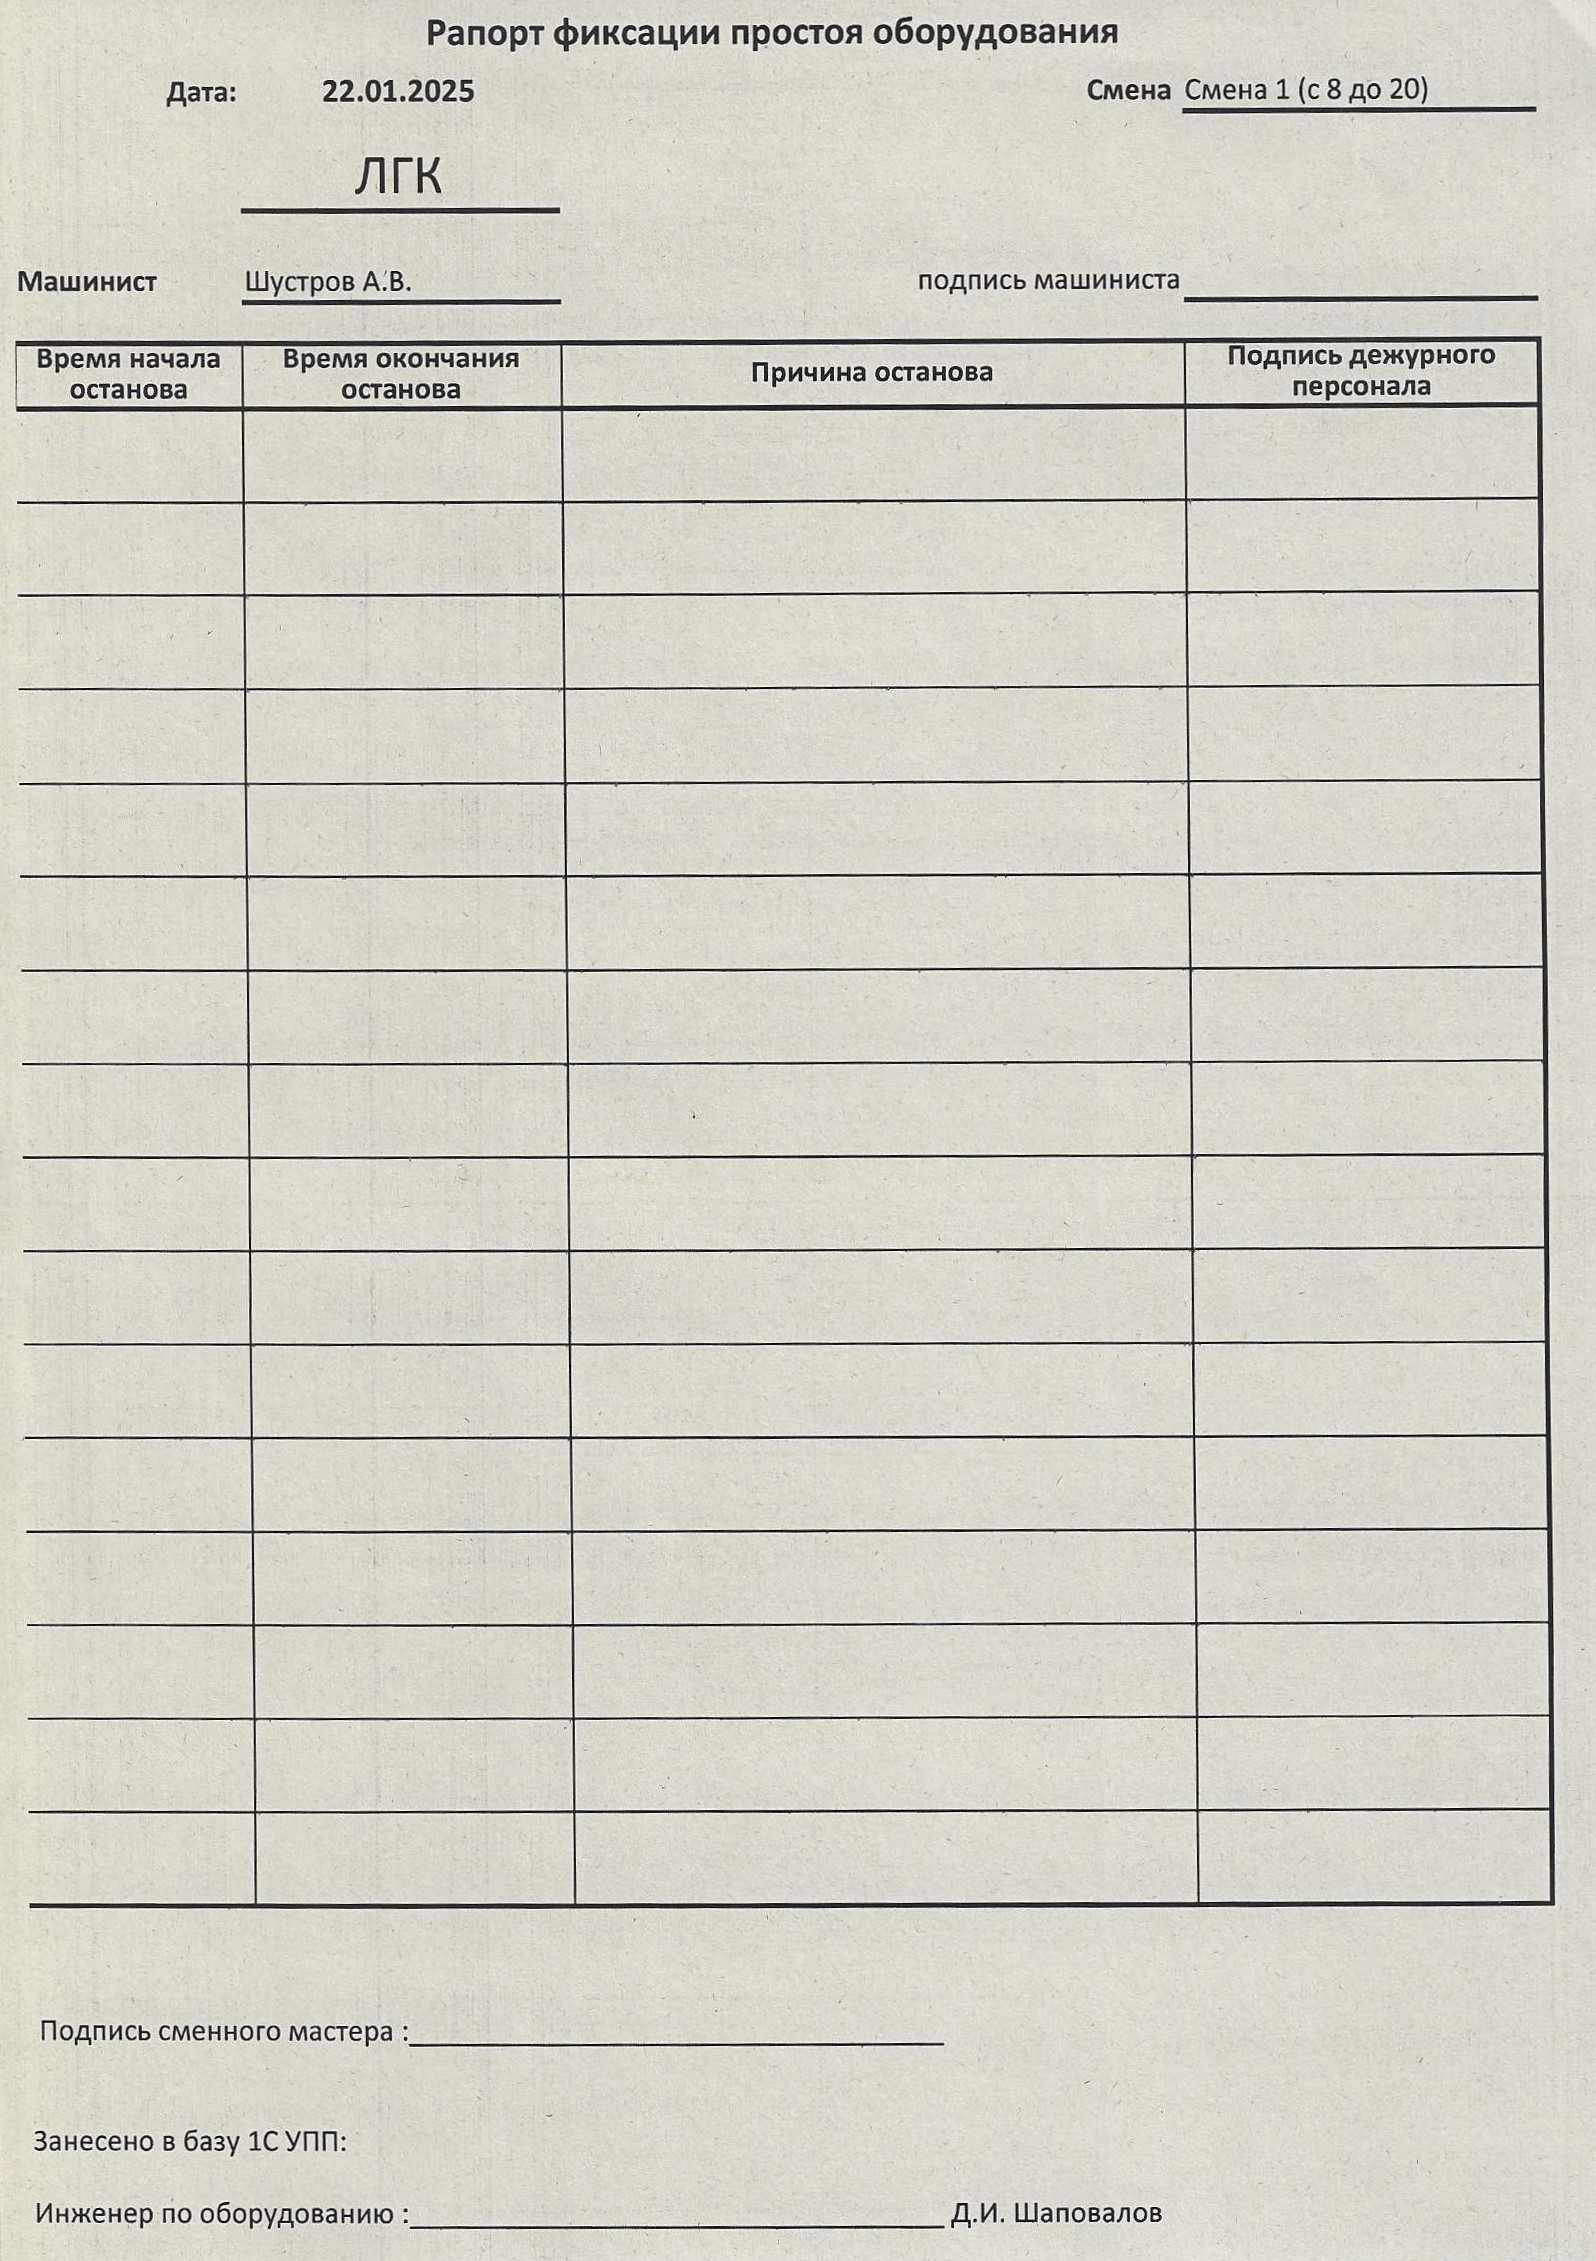
\includegraphics[height=0.9\textheight, keepaspectratio]{Pics/V.9.jpg}
\end{center}
 \caption{Бланк простоев оборудования}
 \label{pic:V.9}
\end{figure}

\begin{figure}
\begin{center}
 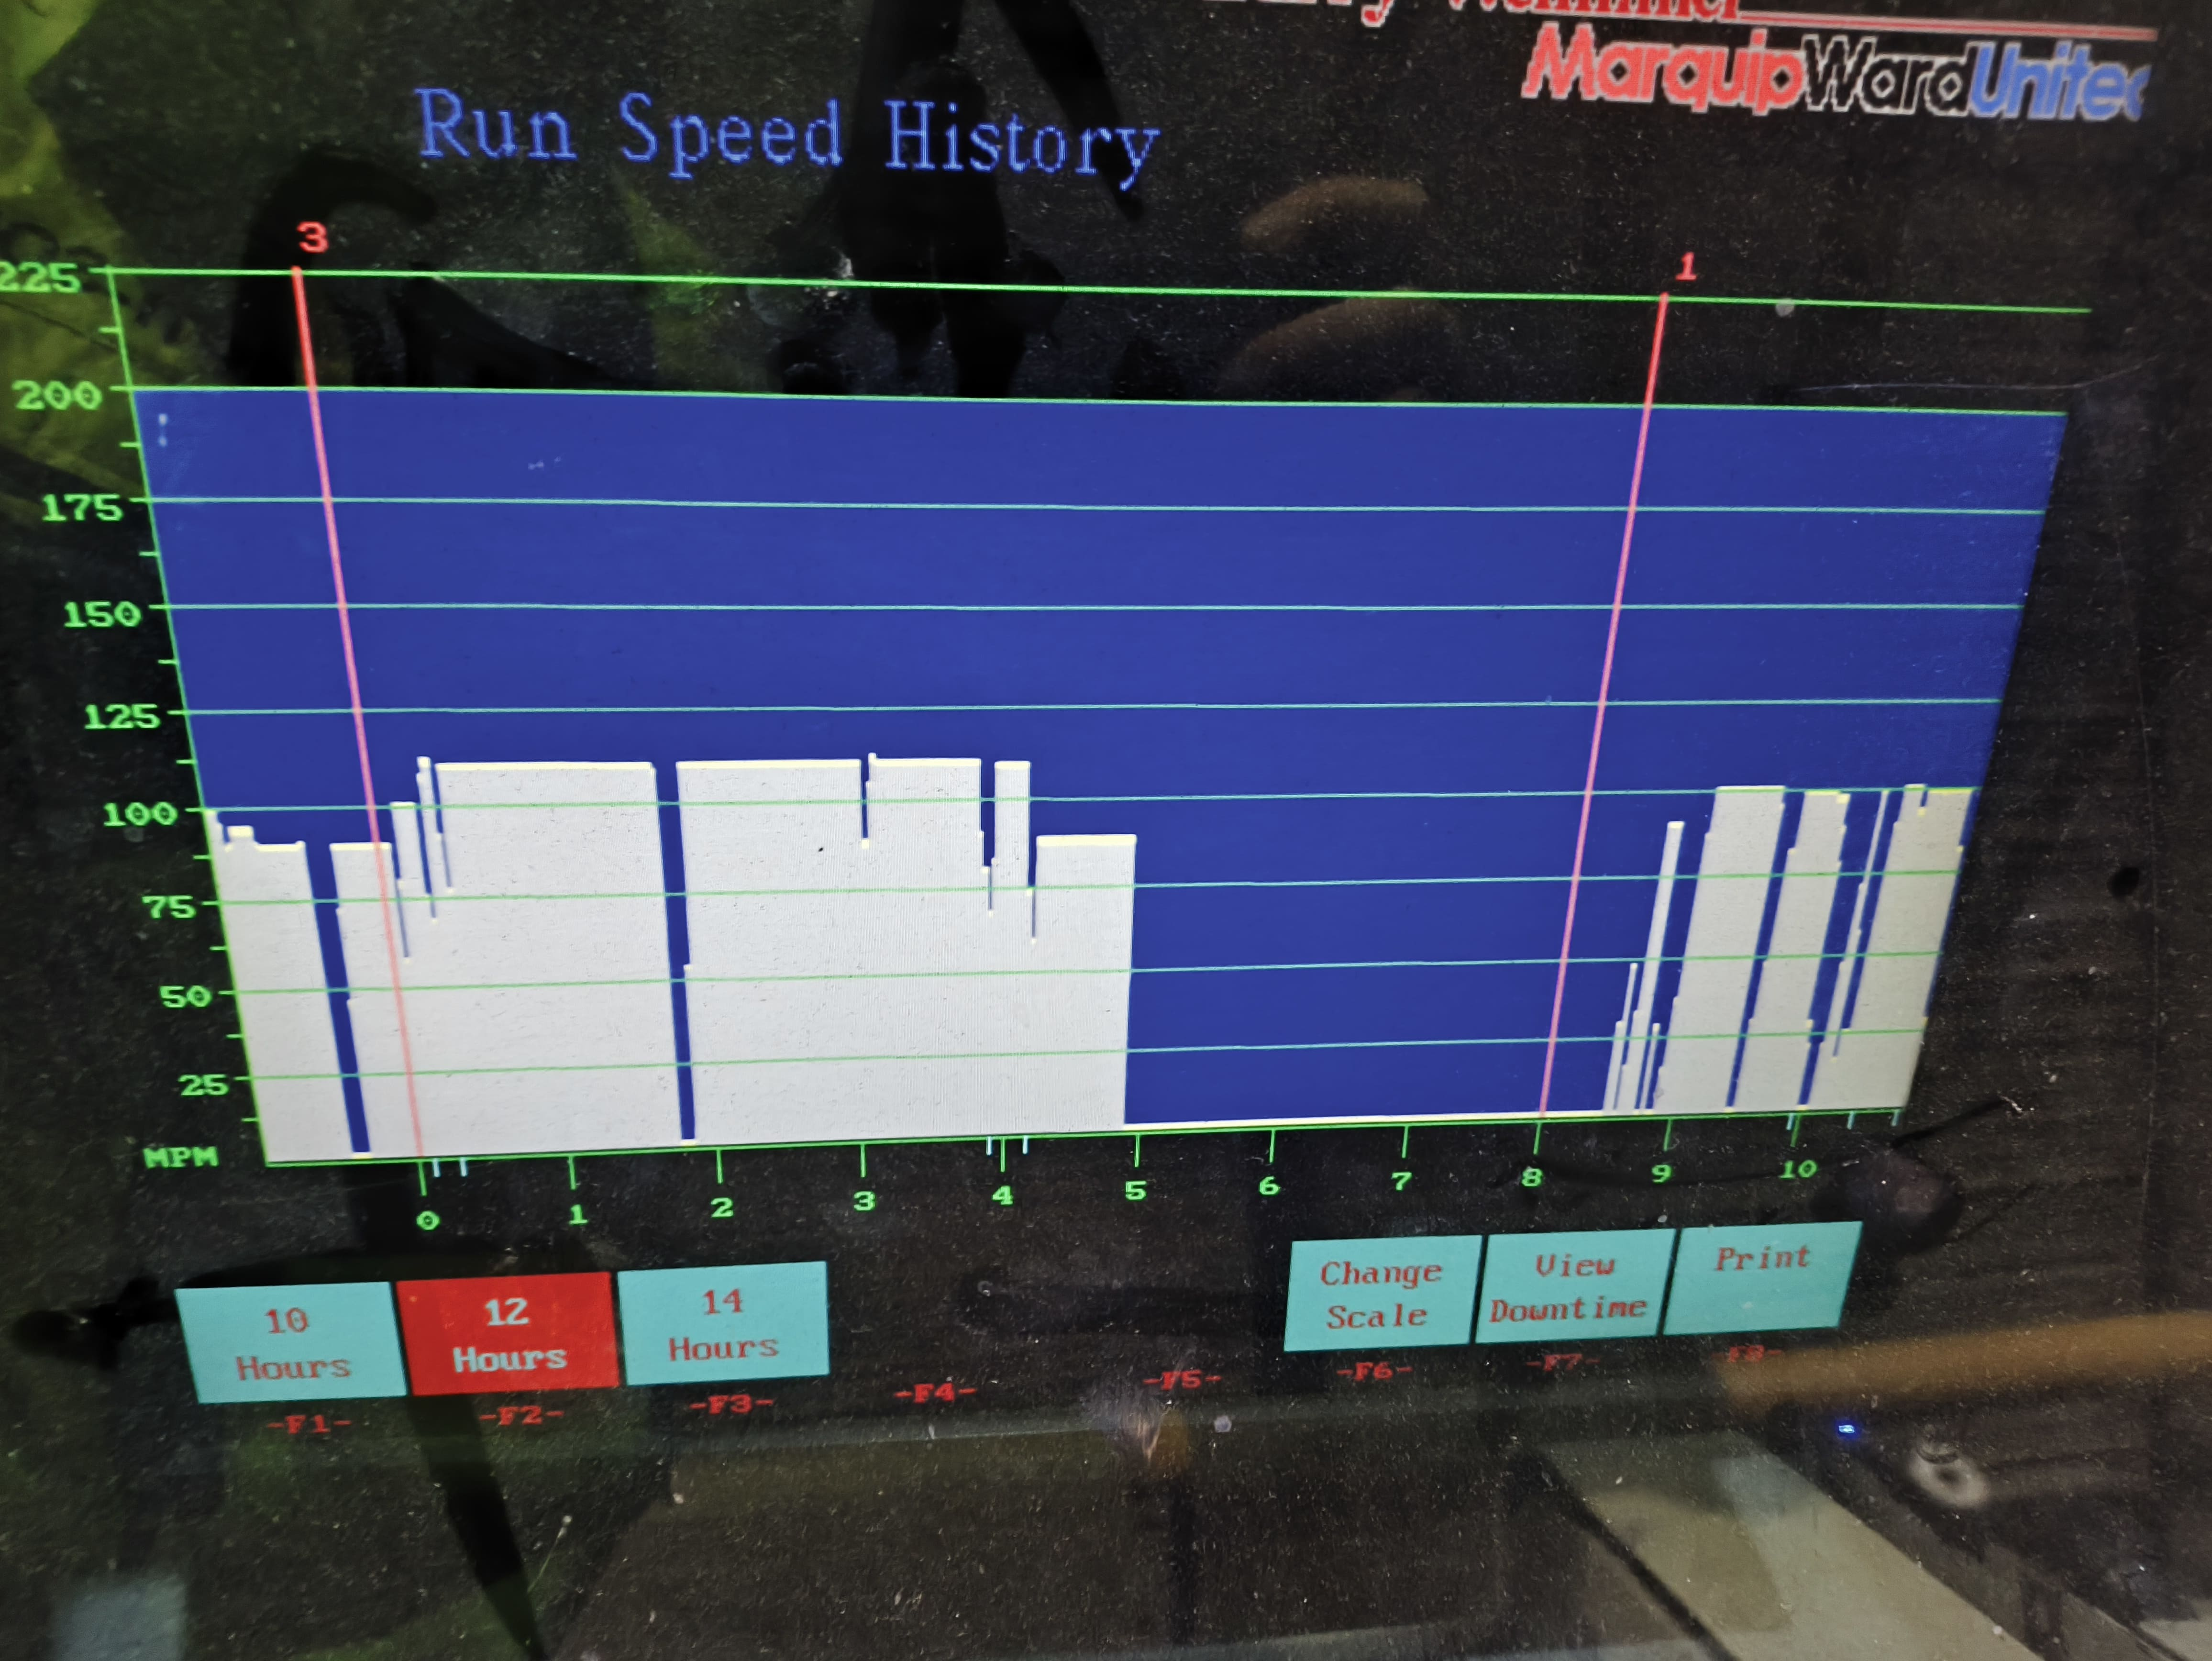
\includegraphics[height=0.5\textheight, keepaspectratio]{Pics/V Остановы ГА.jpg}
\end{center}
 \caption{График работы ЛГК}
 \label{pic:V Остановы ГА}
\end{figure}
%\clearpage

\begin{figure}
\begin{center}
 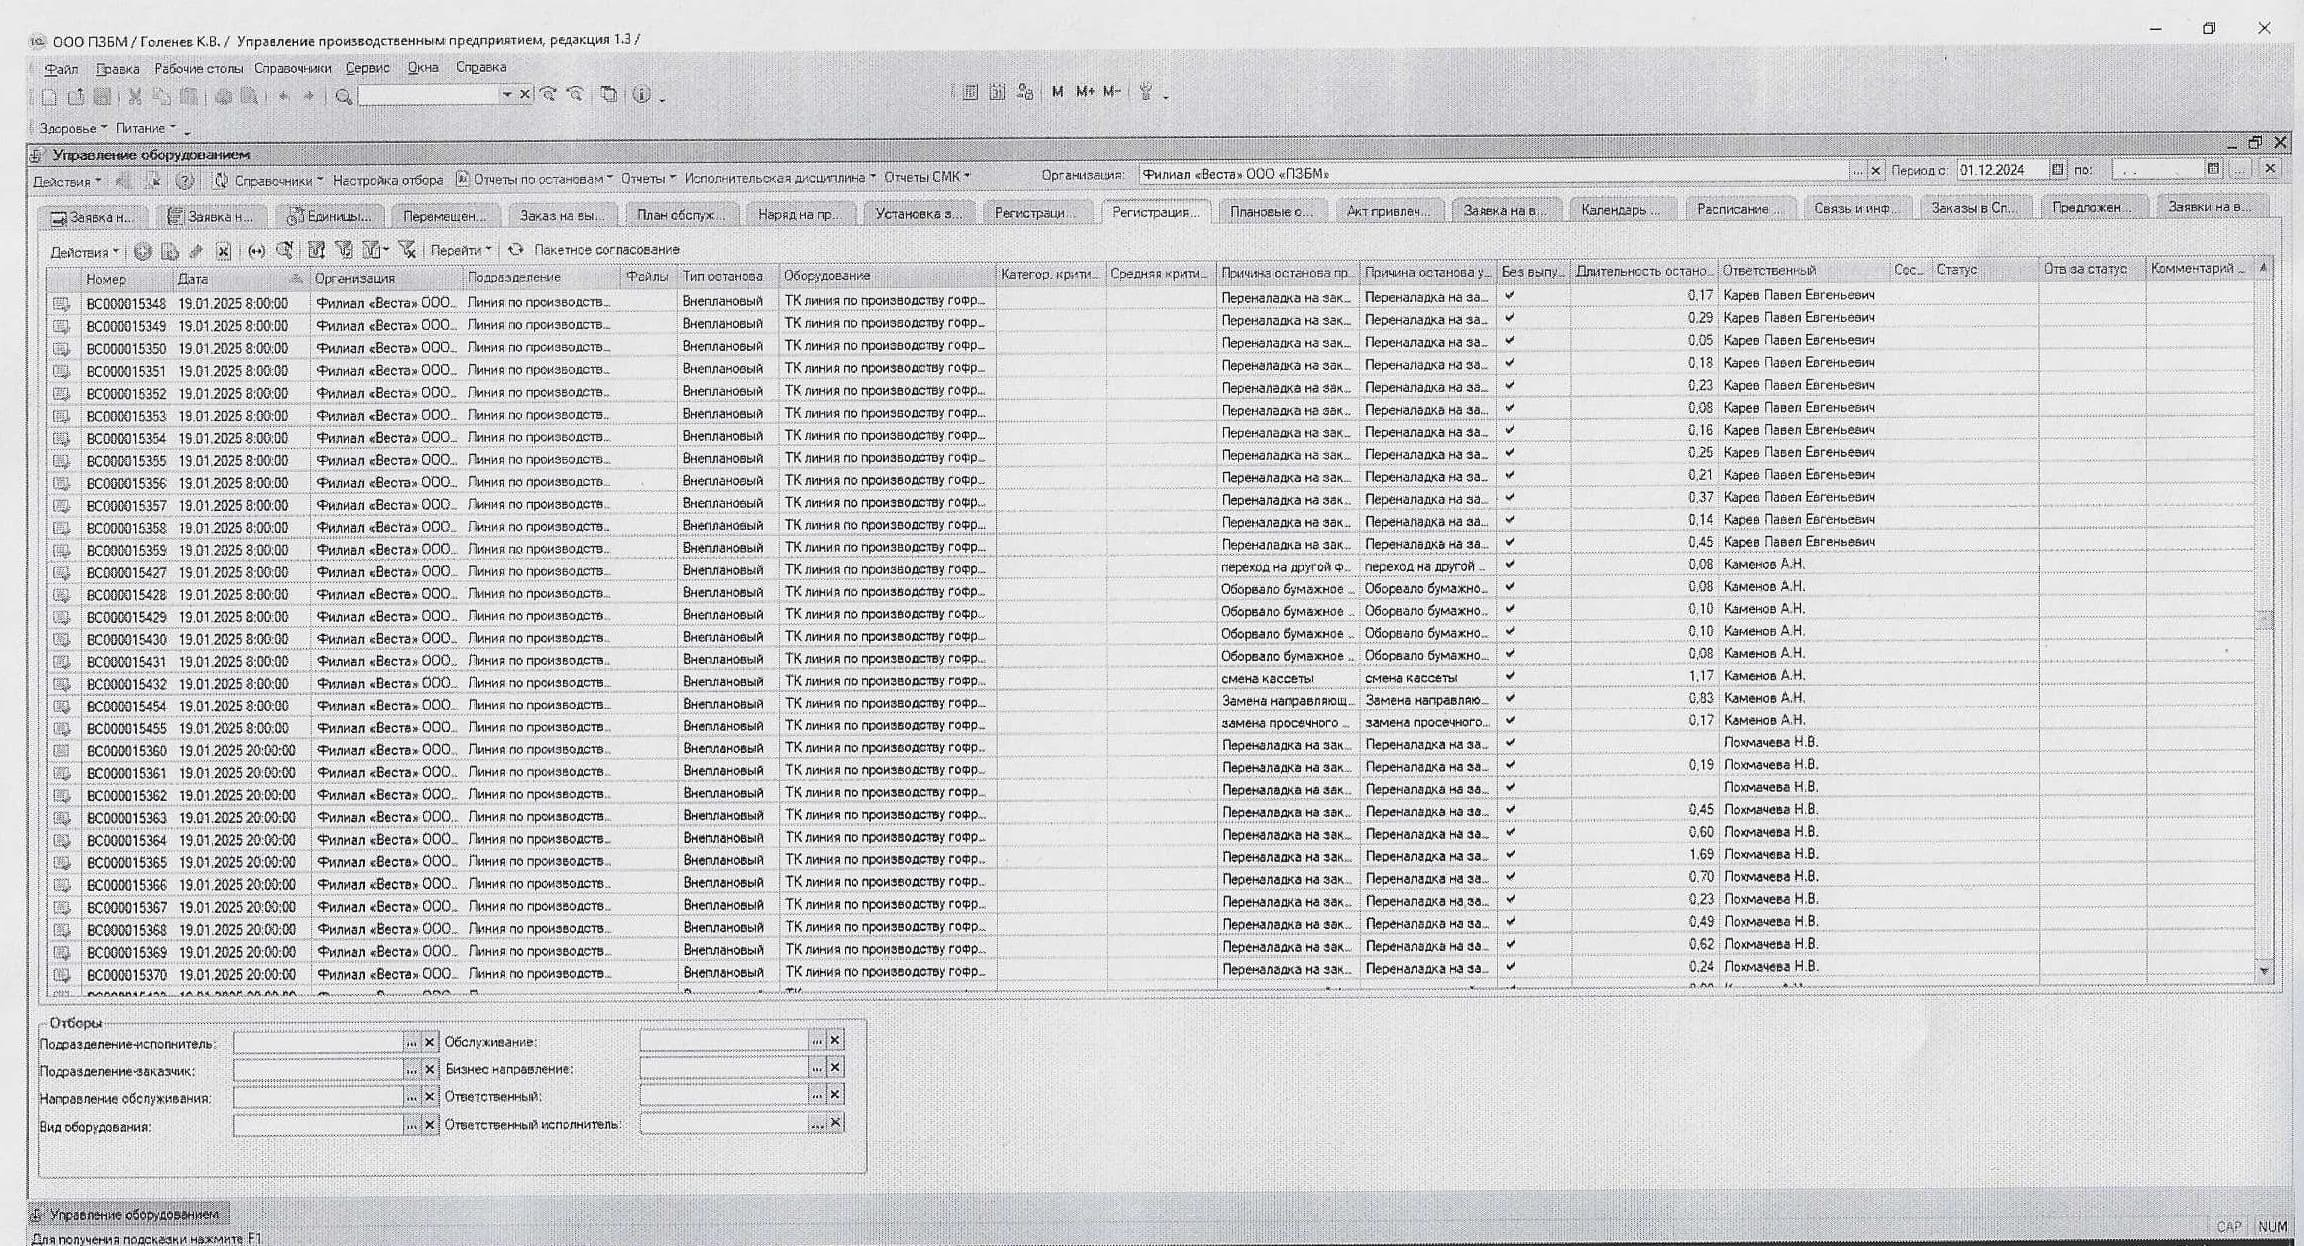
\includegraphics[height=0.37\textheight, keepaspectratio]{Pics/XII.6.jpg}
\end{center}
 \caption{Простои оборудования в 1С: УПП}
 \label{pic:XII.6.jpg}
\end{figure}

\begin{figure}
\begin{center}
 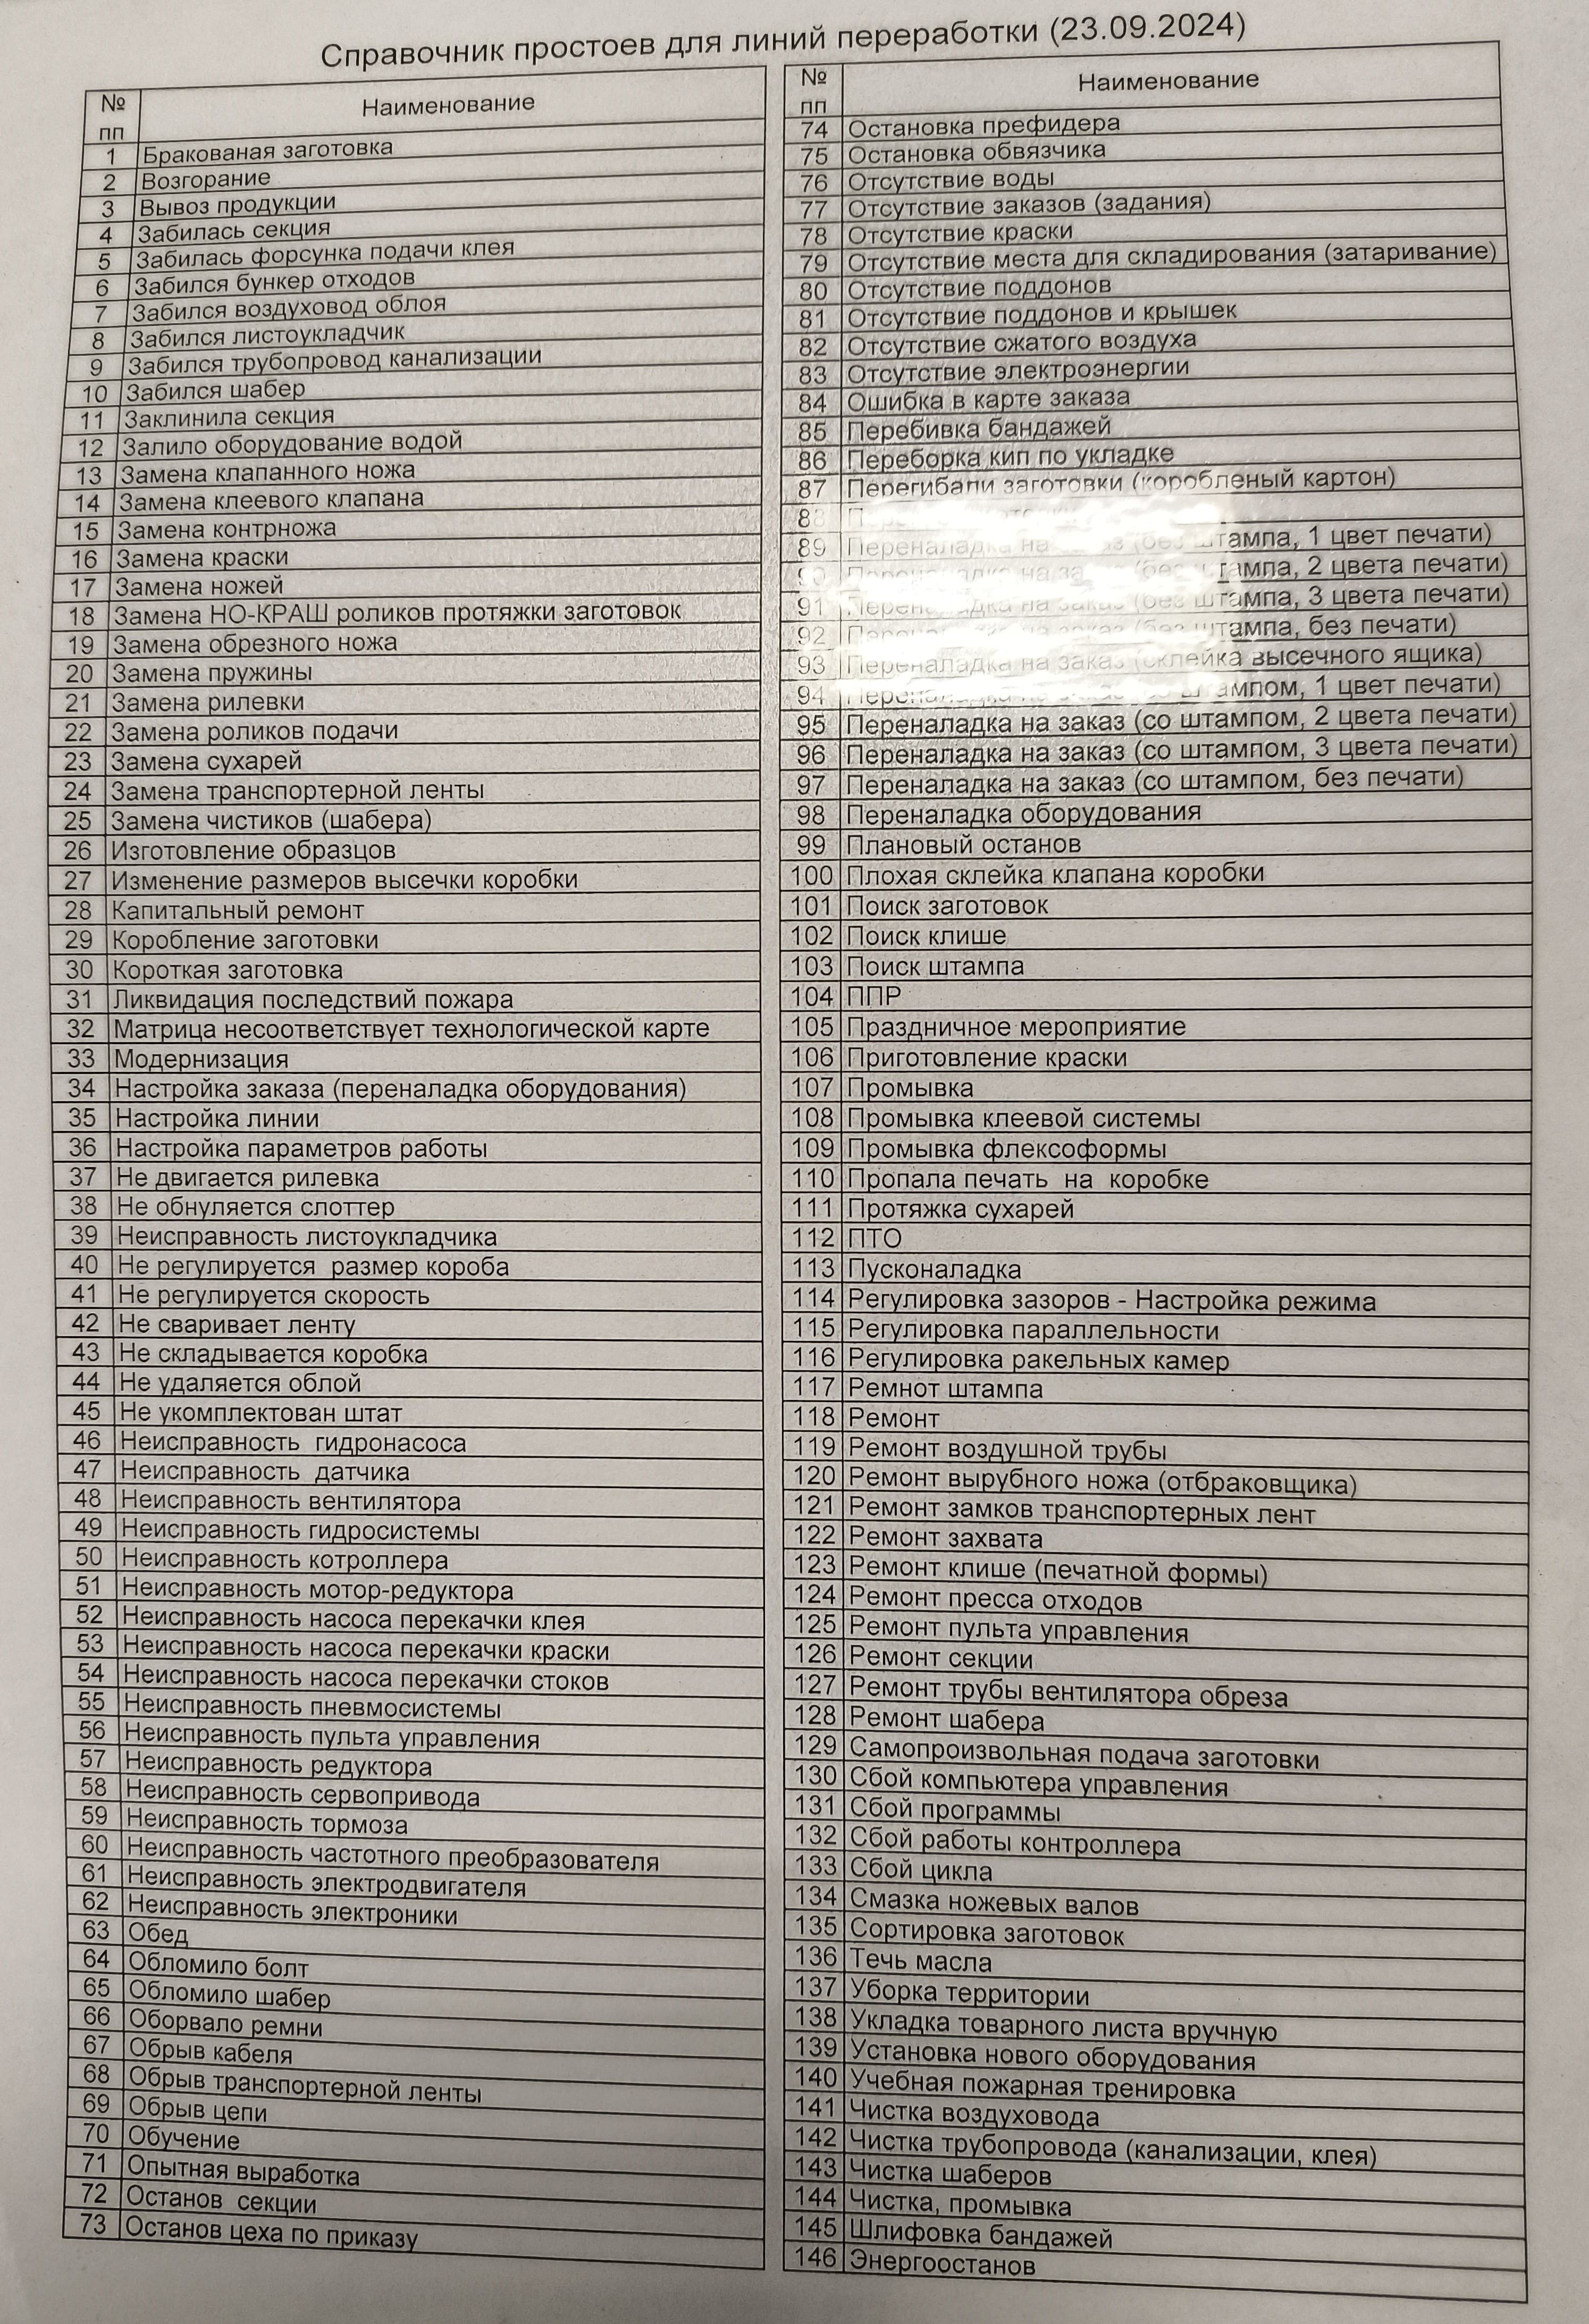
\includegraphics[height=0.9\textheight, keepaspectratio]{Pics/IIIсправочникпростоев.jpg}
\end{center}
 \caption{Справочник простоев}
 \label{pic:IIIсправочникпростоев}
\end{figure}
\clearpage
\begin{figure}
\begin{center}
 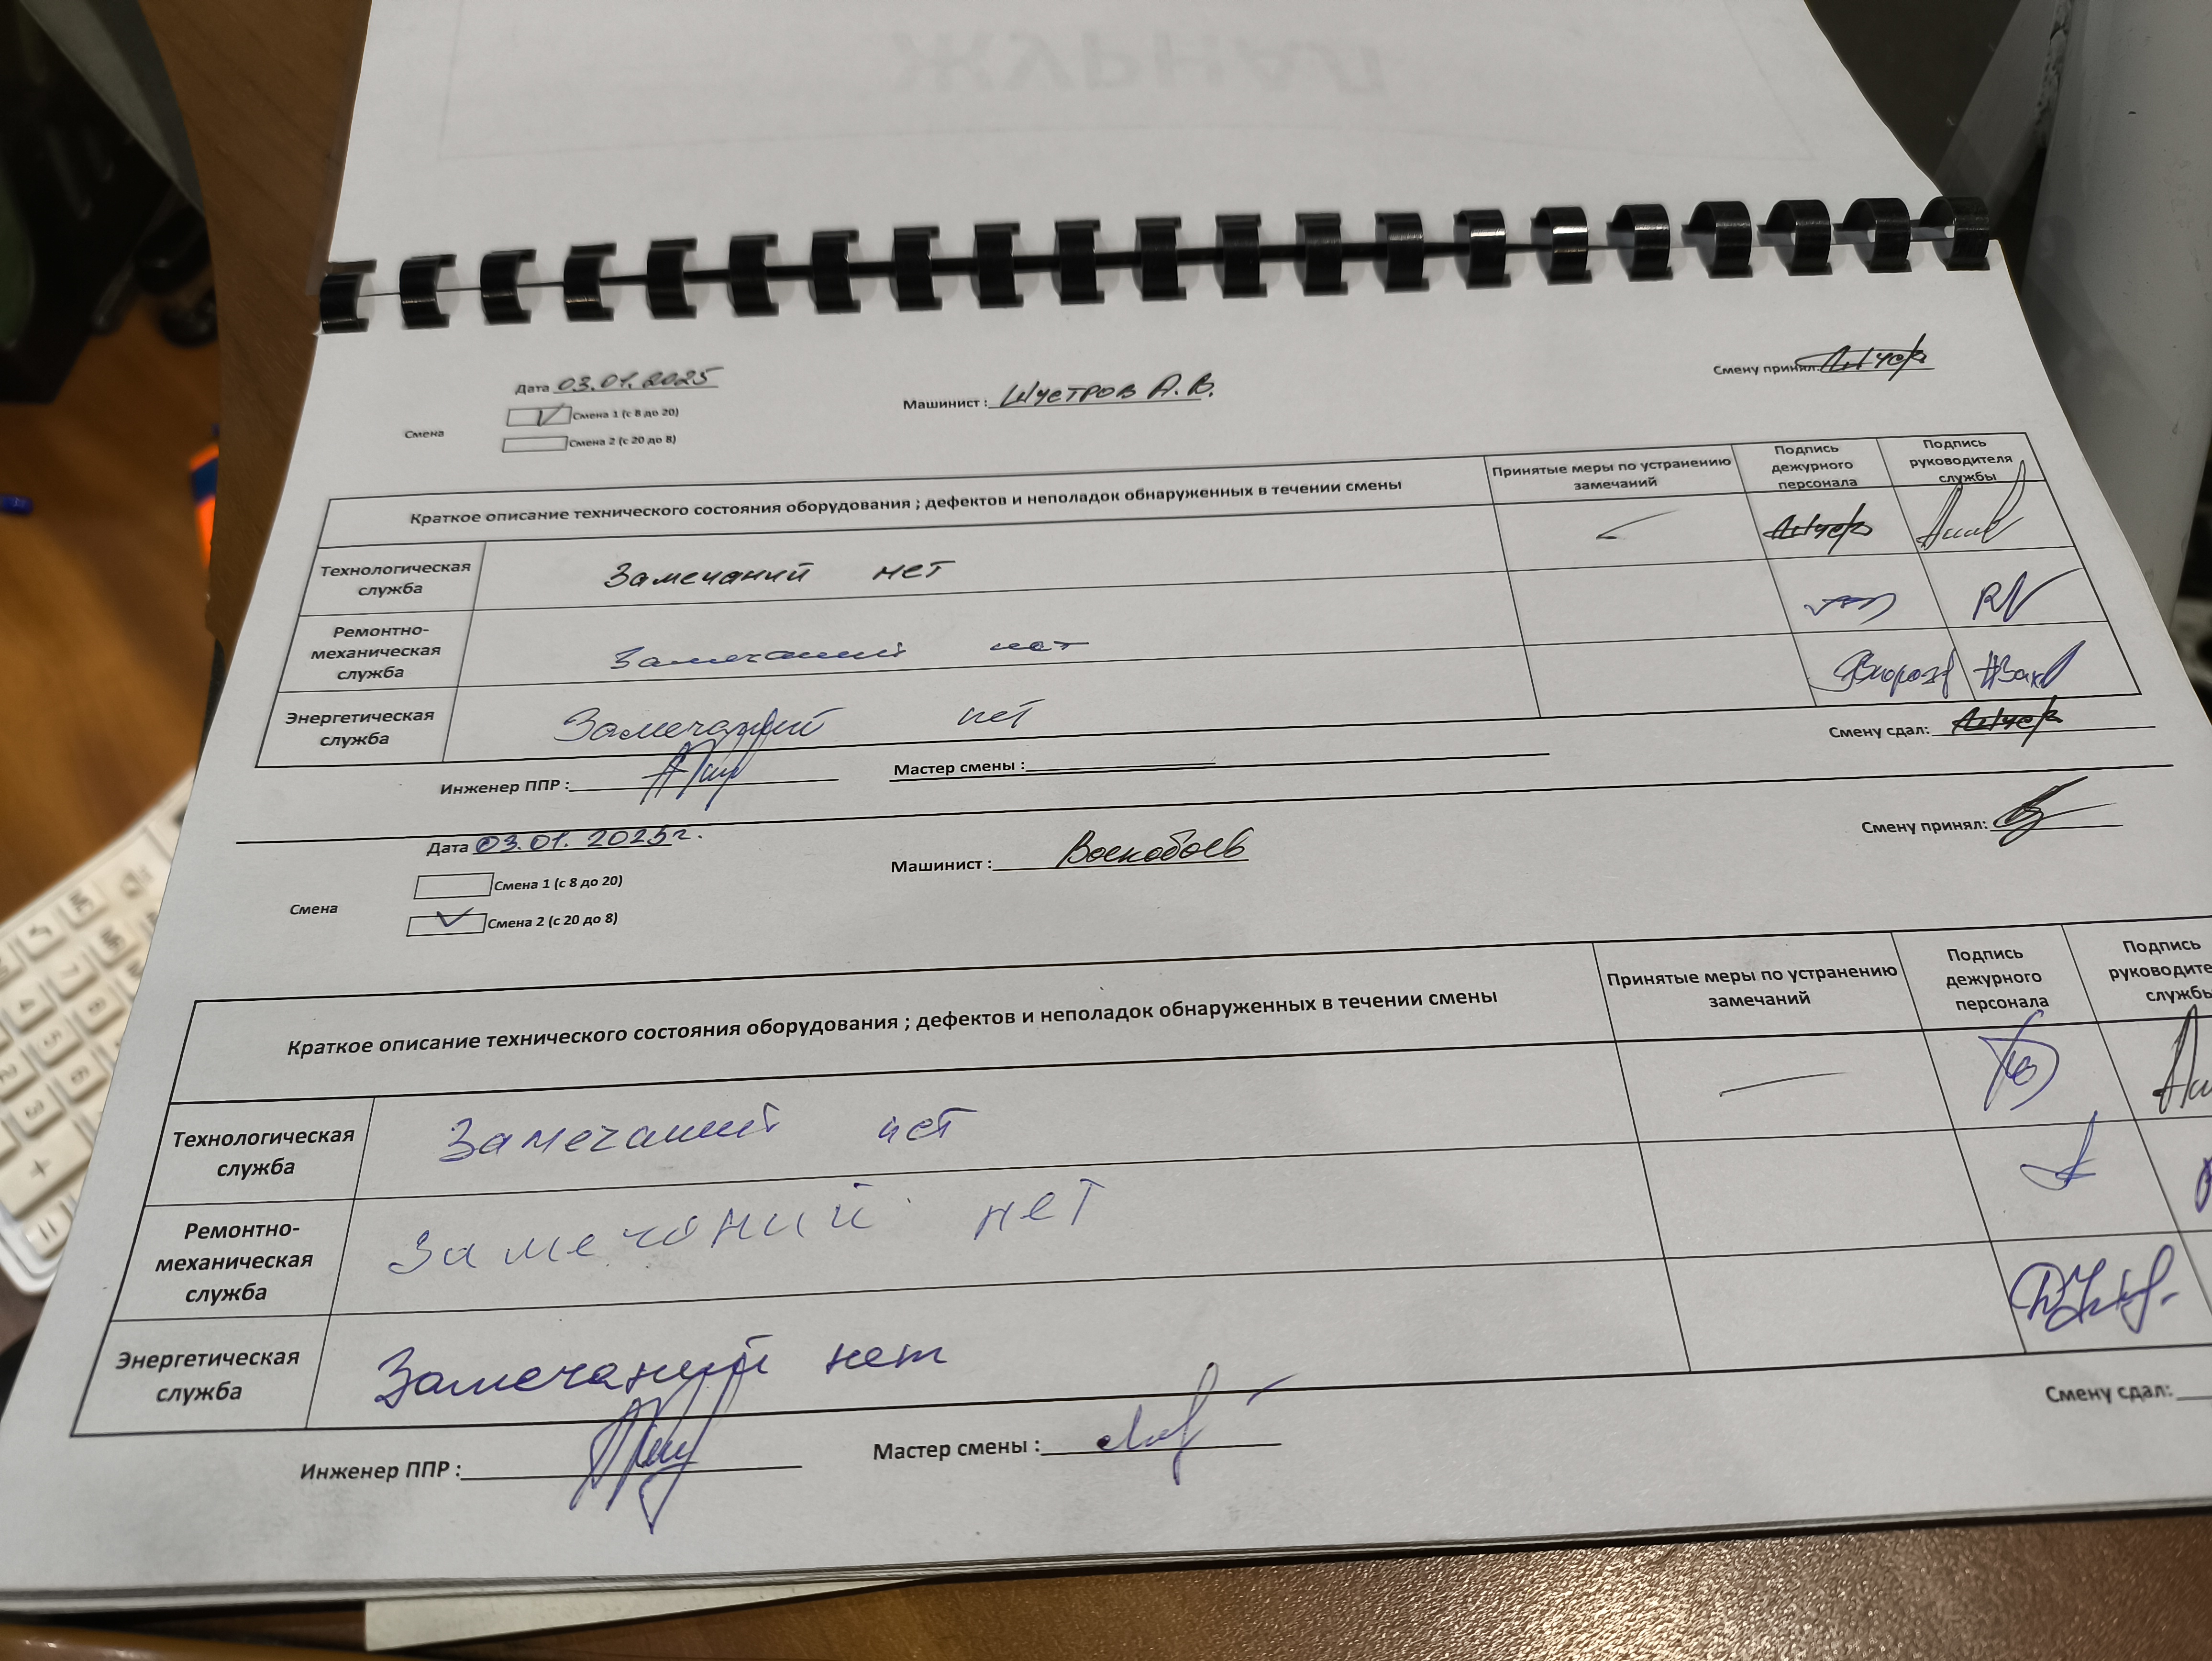
\includegraphics[height=0.5\textheight, keepaspectratio]{Pics/VжурналнаГА2.jpg}
\end{center}
 \caption{Сменный журнал}
 \label{pic:VжурналнаГА2}
\end{figure}

%\begin{figure}
%\begin{center}
 %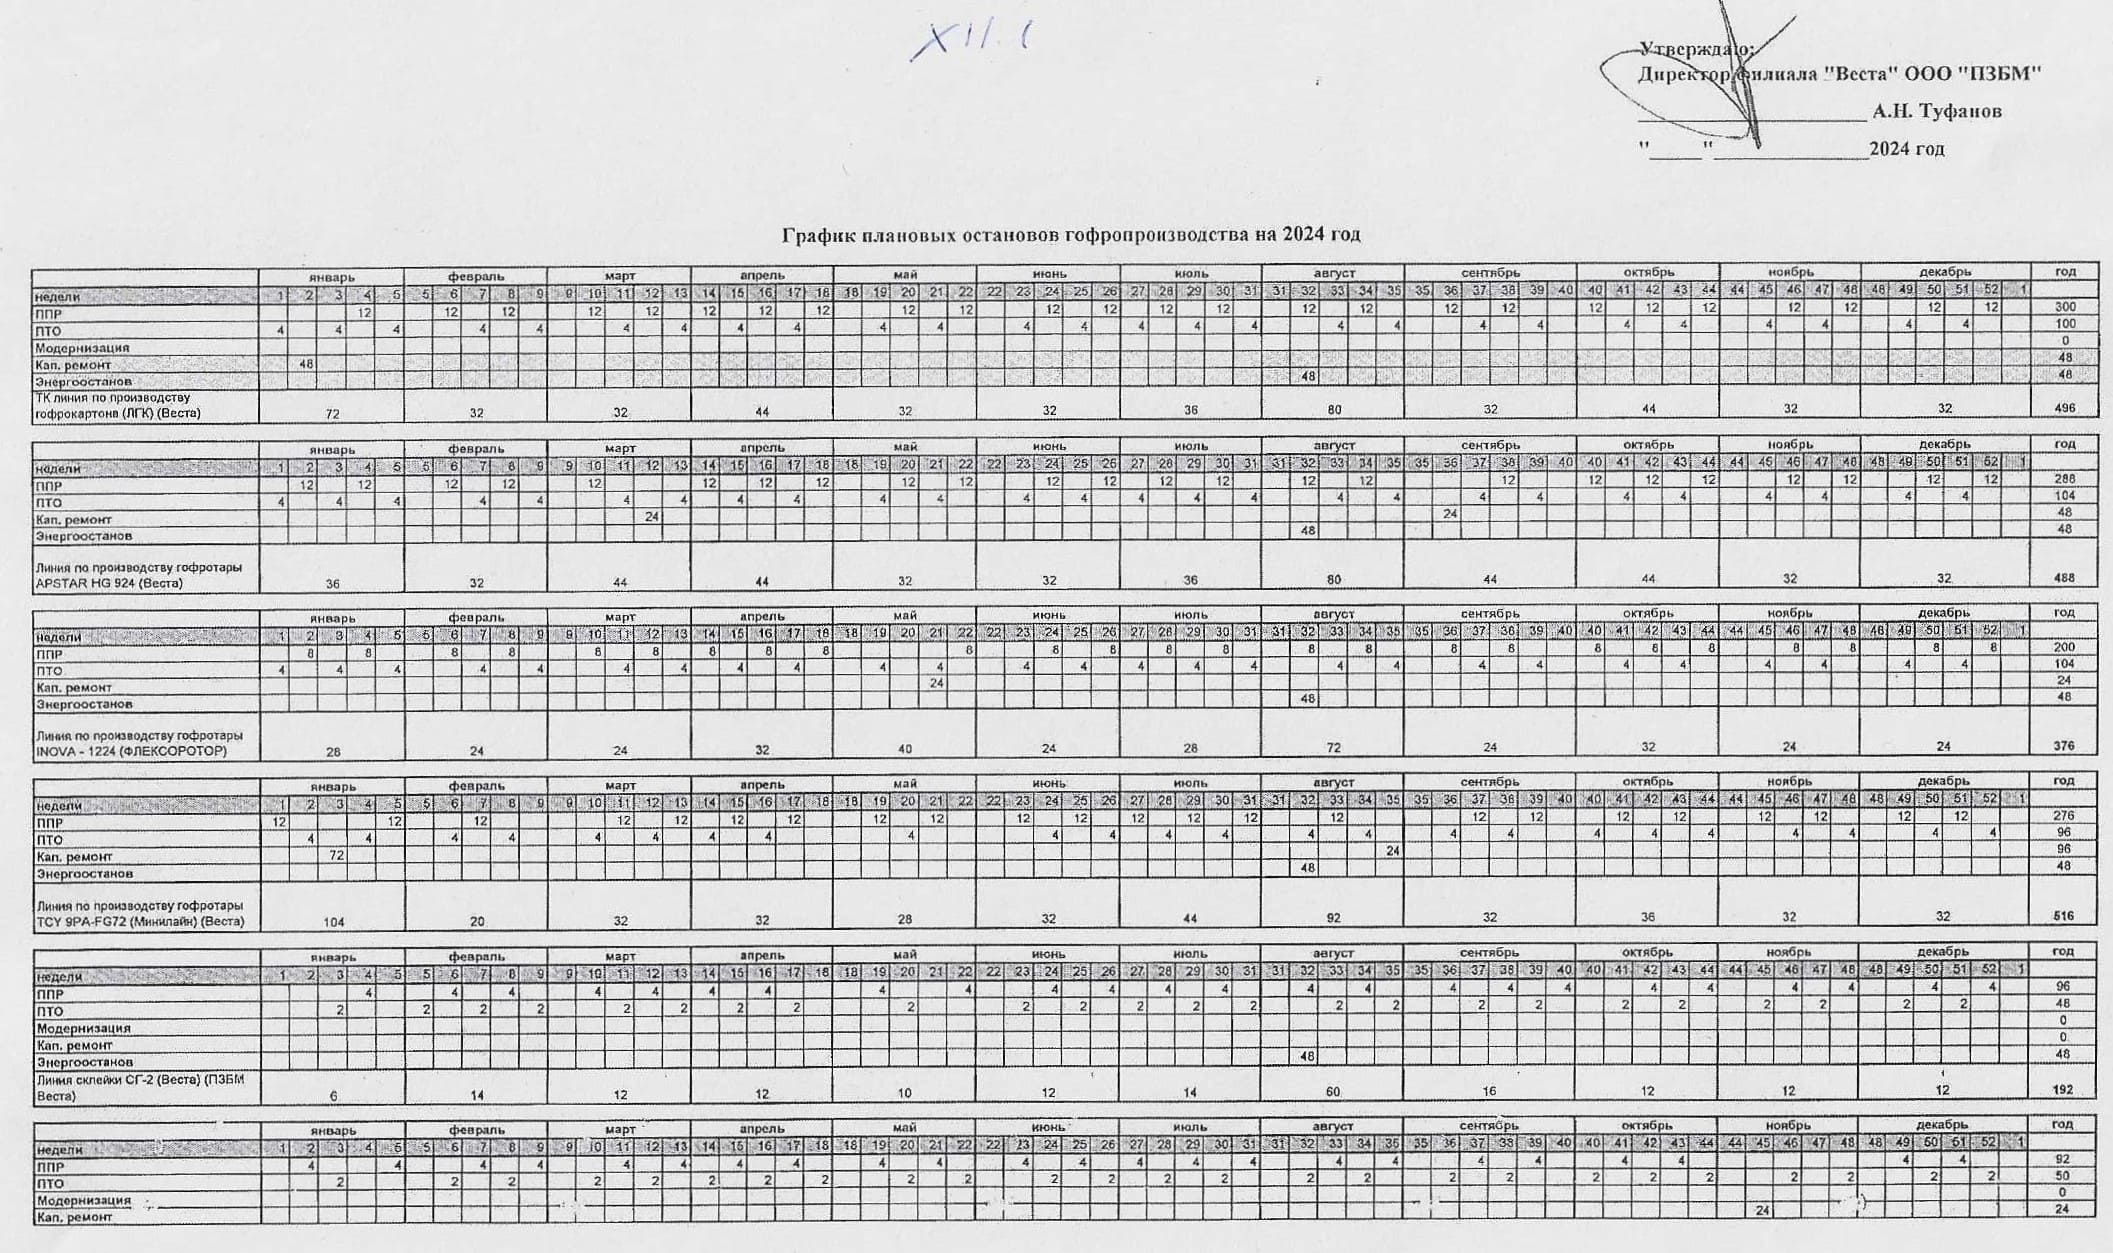
\includegraphics[height=0.4\textheight, keepaspectratio]{Pics/XII.1.jpg}
%\end{center}
 %\caption{Годовой график остановов}
 %\label{pic:XII.1.jpg}
%\end{figure}

\begin{figure}
\begin{center}
 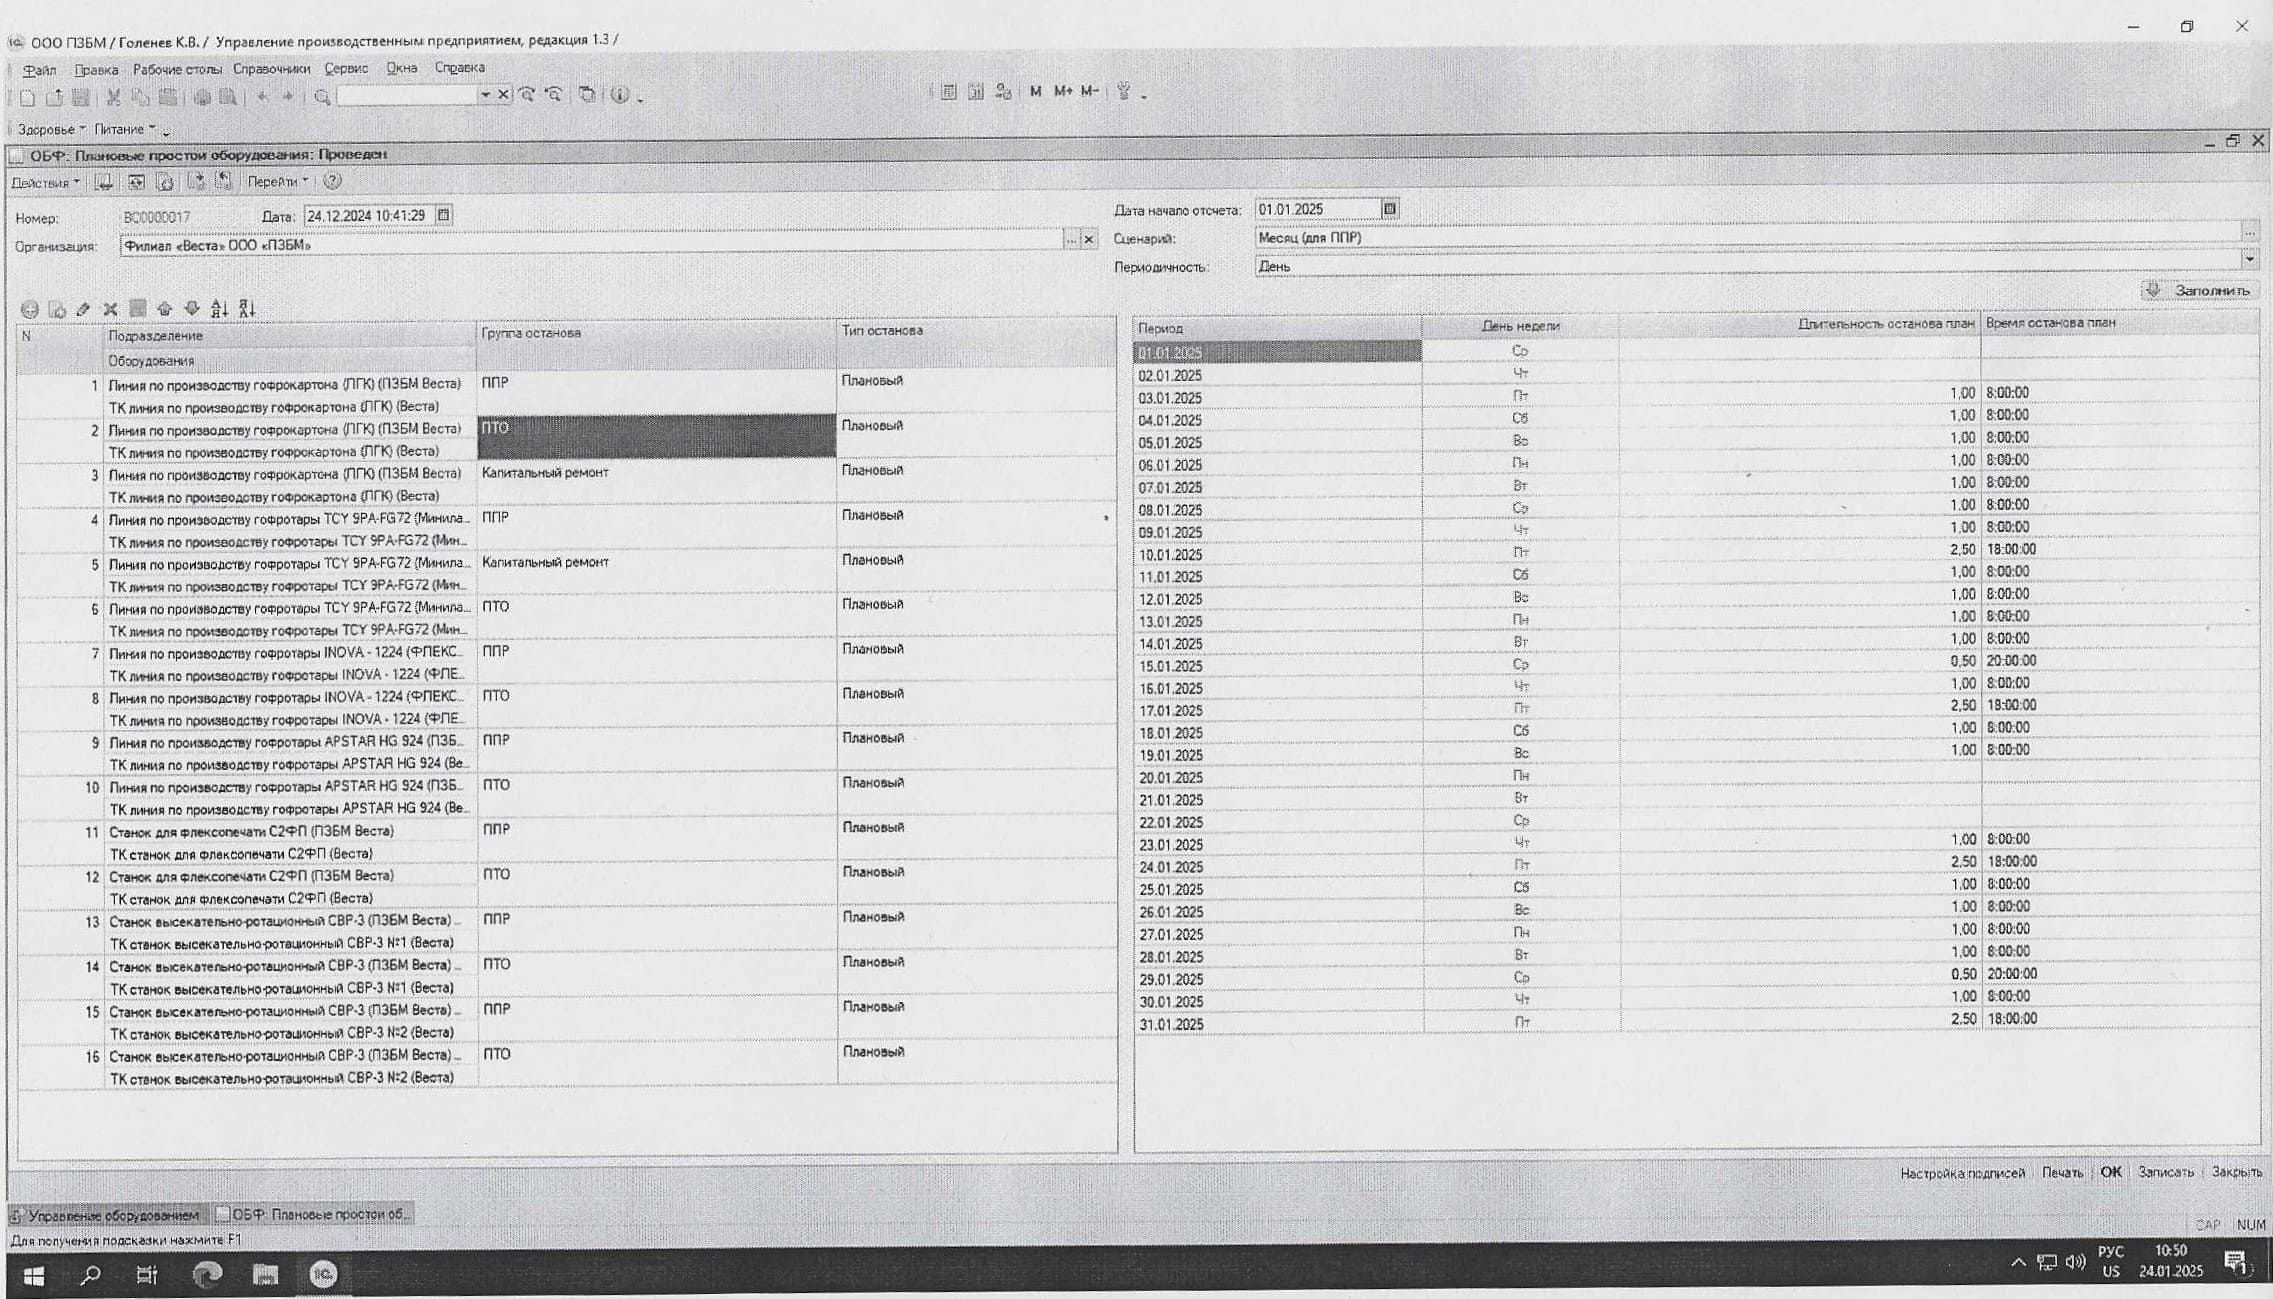
\includegraphics[height=0.39\textheight, keepaspectratio]{Pics/XII.2..jpg}
\end{center}
 \caption{Месячный график ППР}
 \label{pic:XII.2..jpg}
\end{figure}

\begin{figure}
\begin{center}
 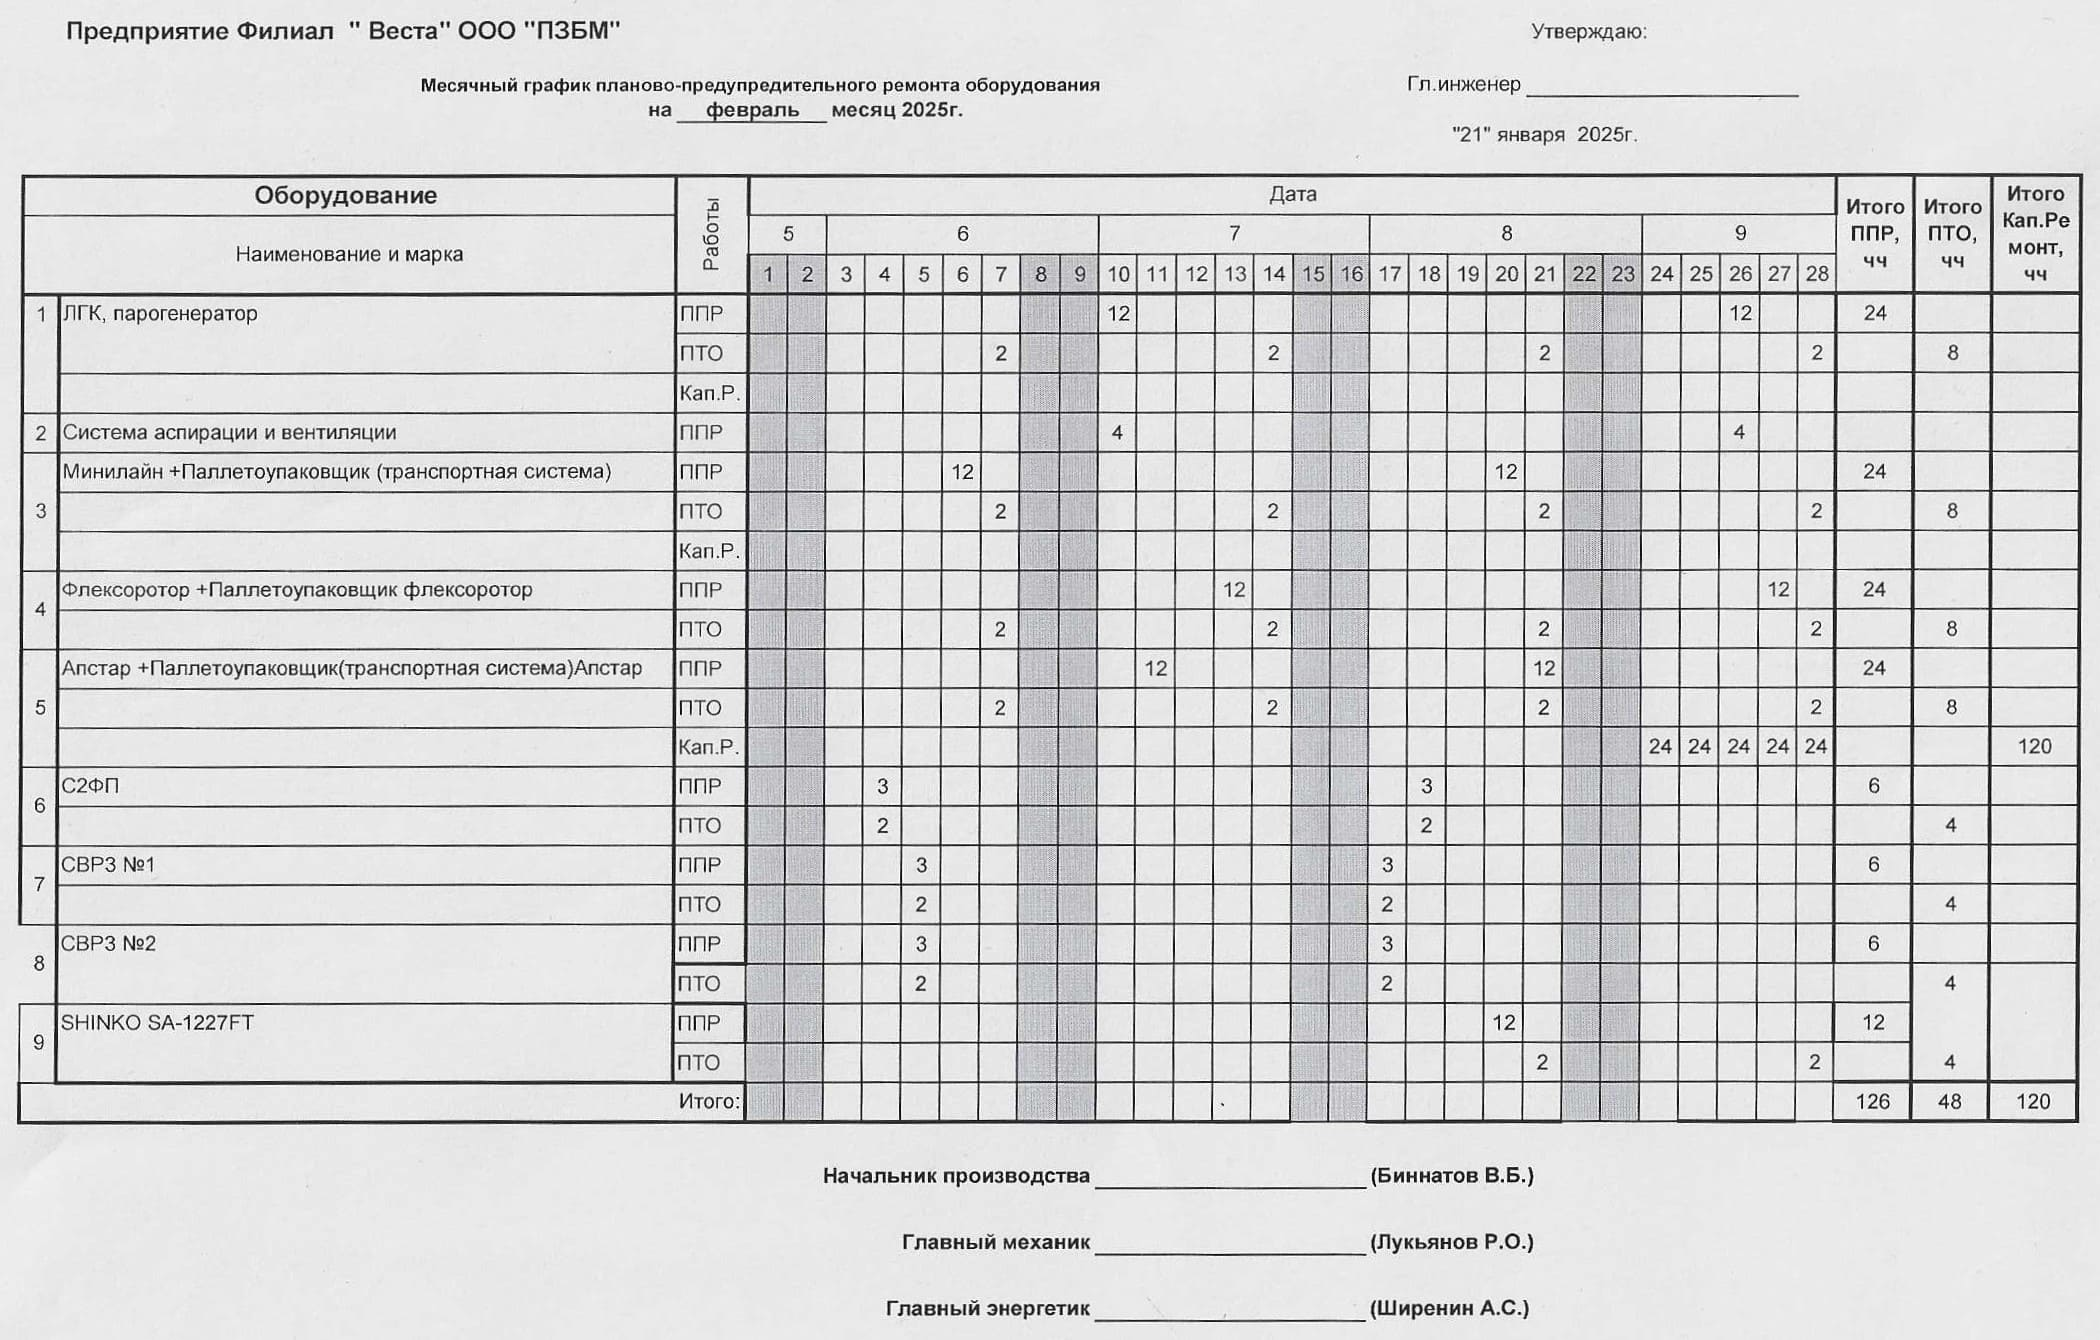
\includegraphics[height=0.4\textheight, keepaspectratio]{Pics/XII.2.jpg}
\end{center}
 \caption{Информация по остановам в 1С: УПП}
 \label{pic:XII.2.jpg}
\end{figure}

\begin{figure}
\begin{center}
 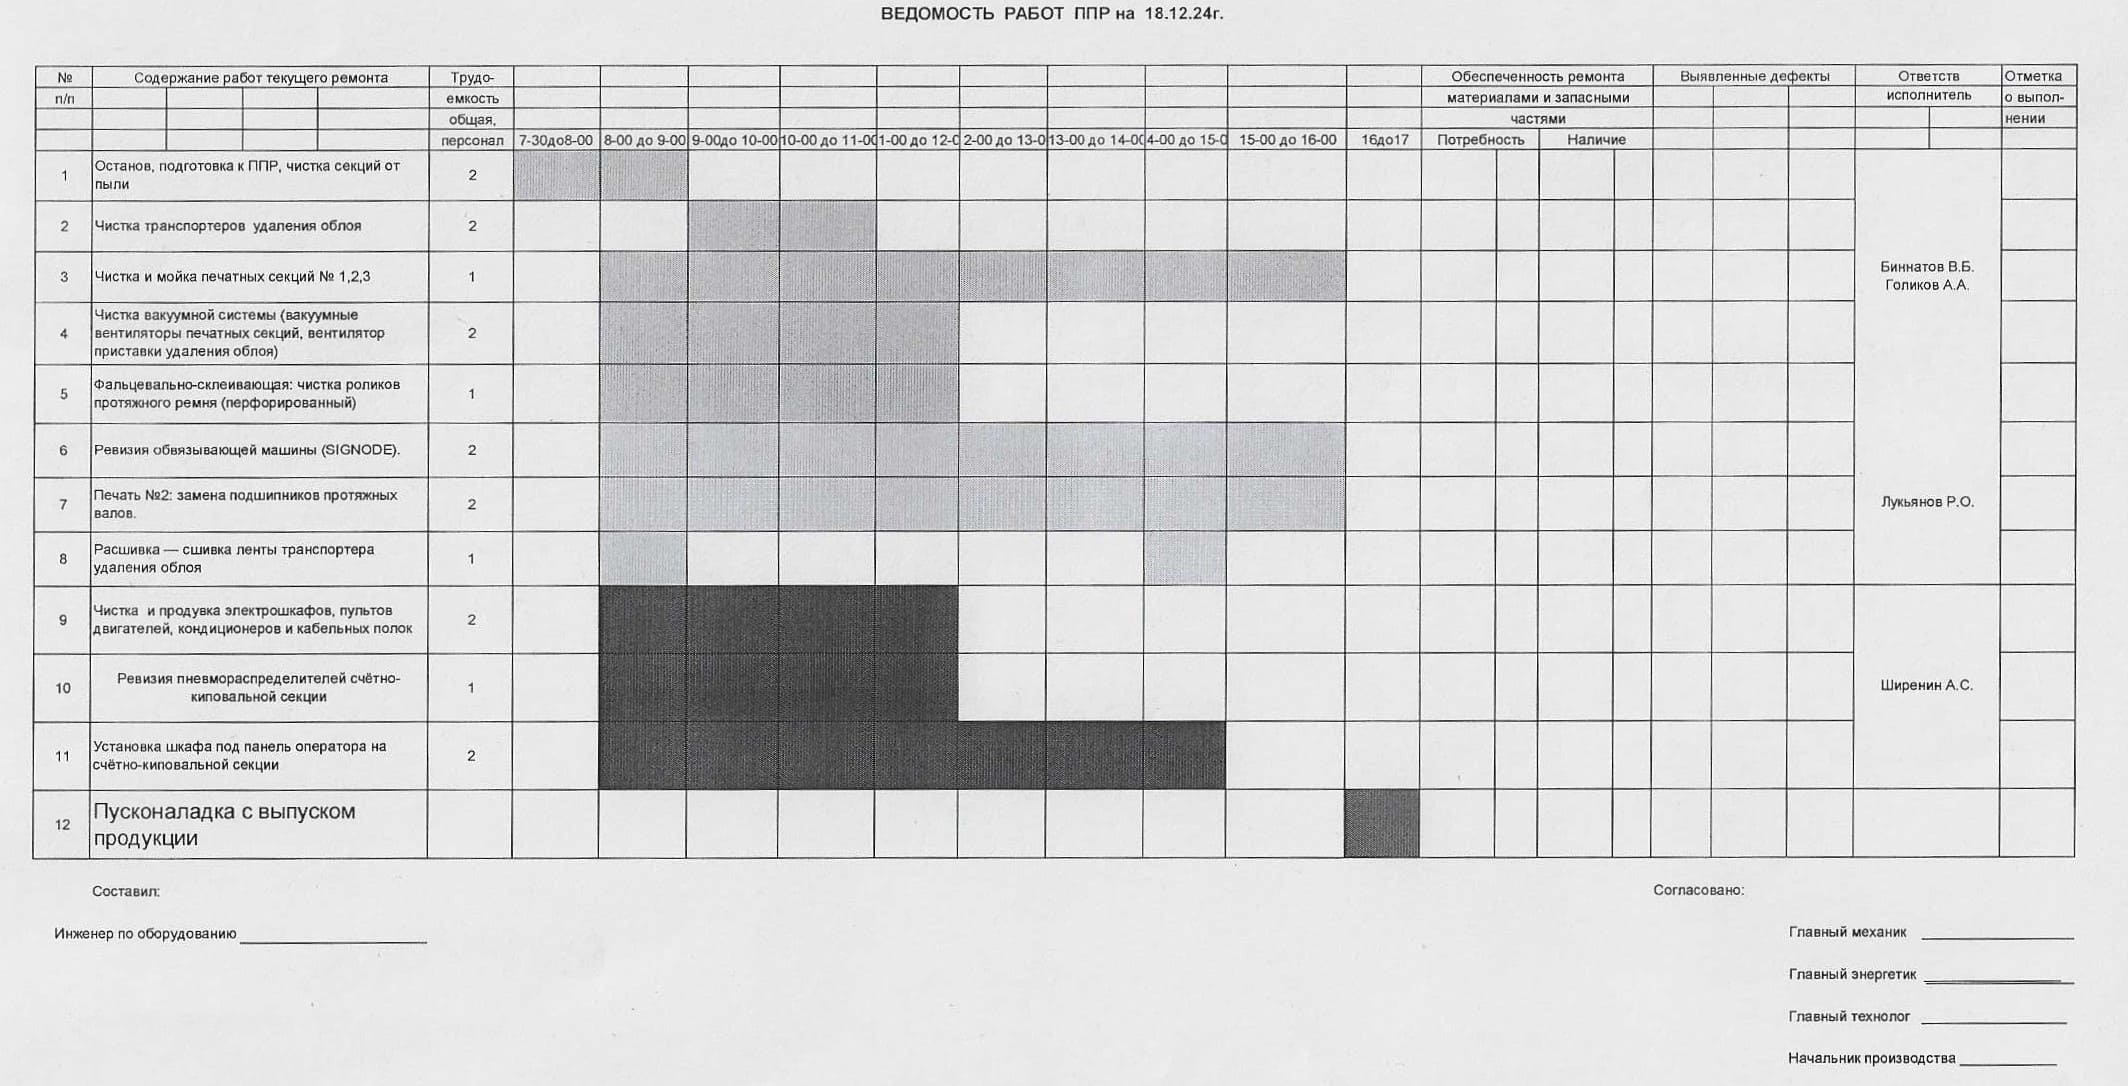
\includegraphics[height=0.35\textheight, keepaspectratio]{Pics/XII.3.jpg}
\end{center}
 \caption{Ведомость работ}
 \label{pic:XII.3.jpg}
\end{figure}

\begin{figure}
\begin{center}
 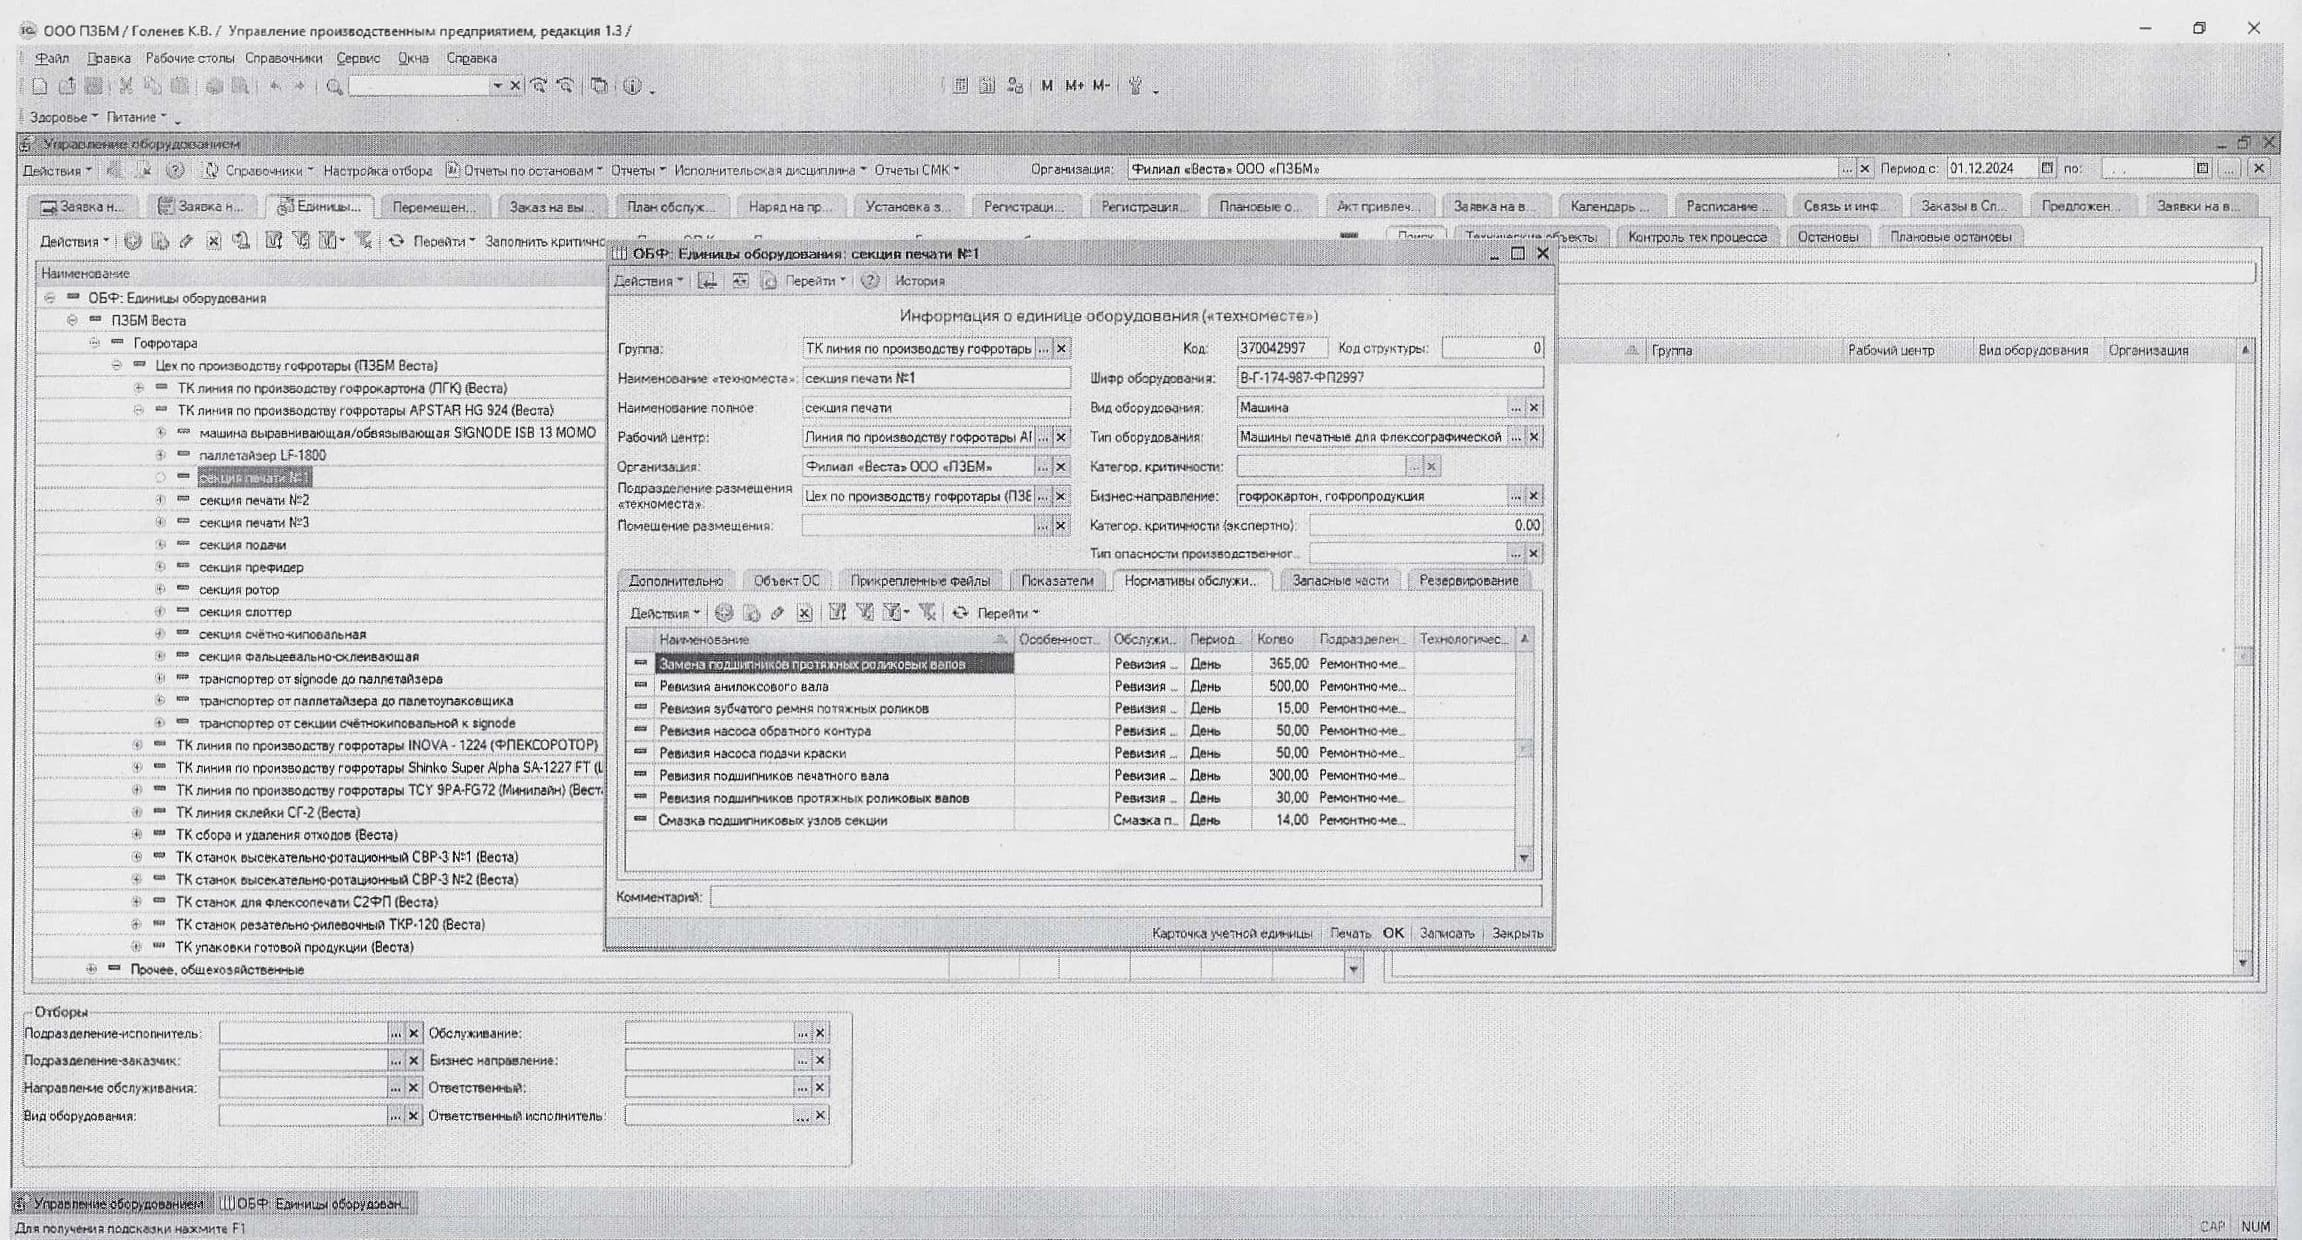
\includegraphics[height=0.37\textheight, keepaspectratio]{Pics/XII.4.jpg}
\end{center}
 \caption{Задание на выполнение работ при проведении ППР}
 \label{pic:XII.4.jpg}
\end{figure}

\begin{figure}
\begin{center}
 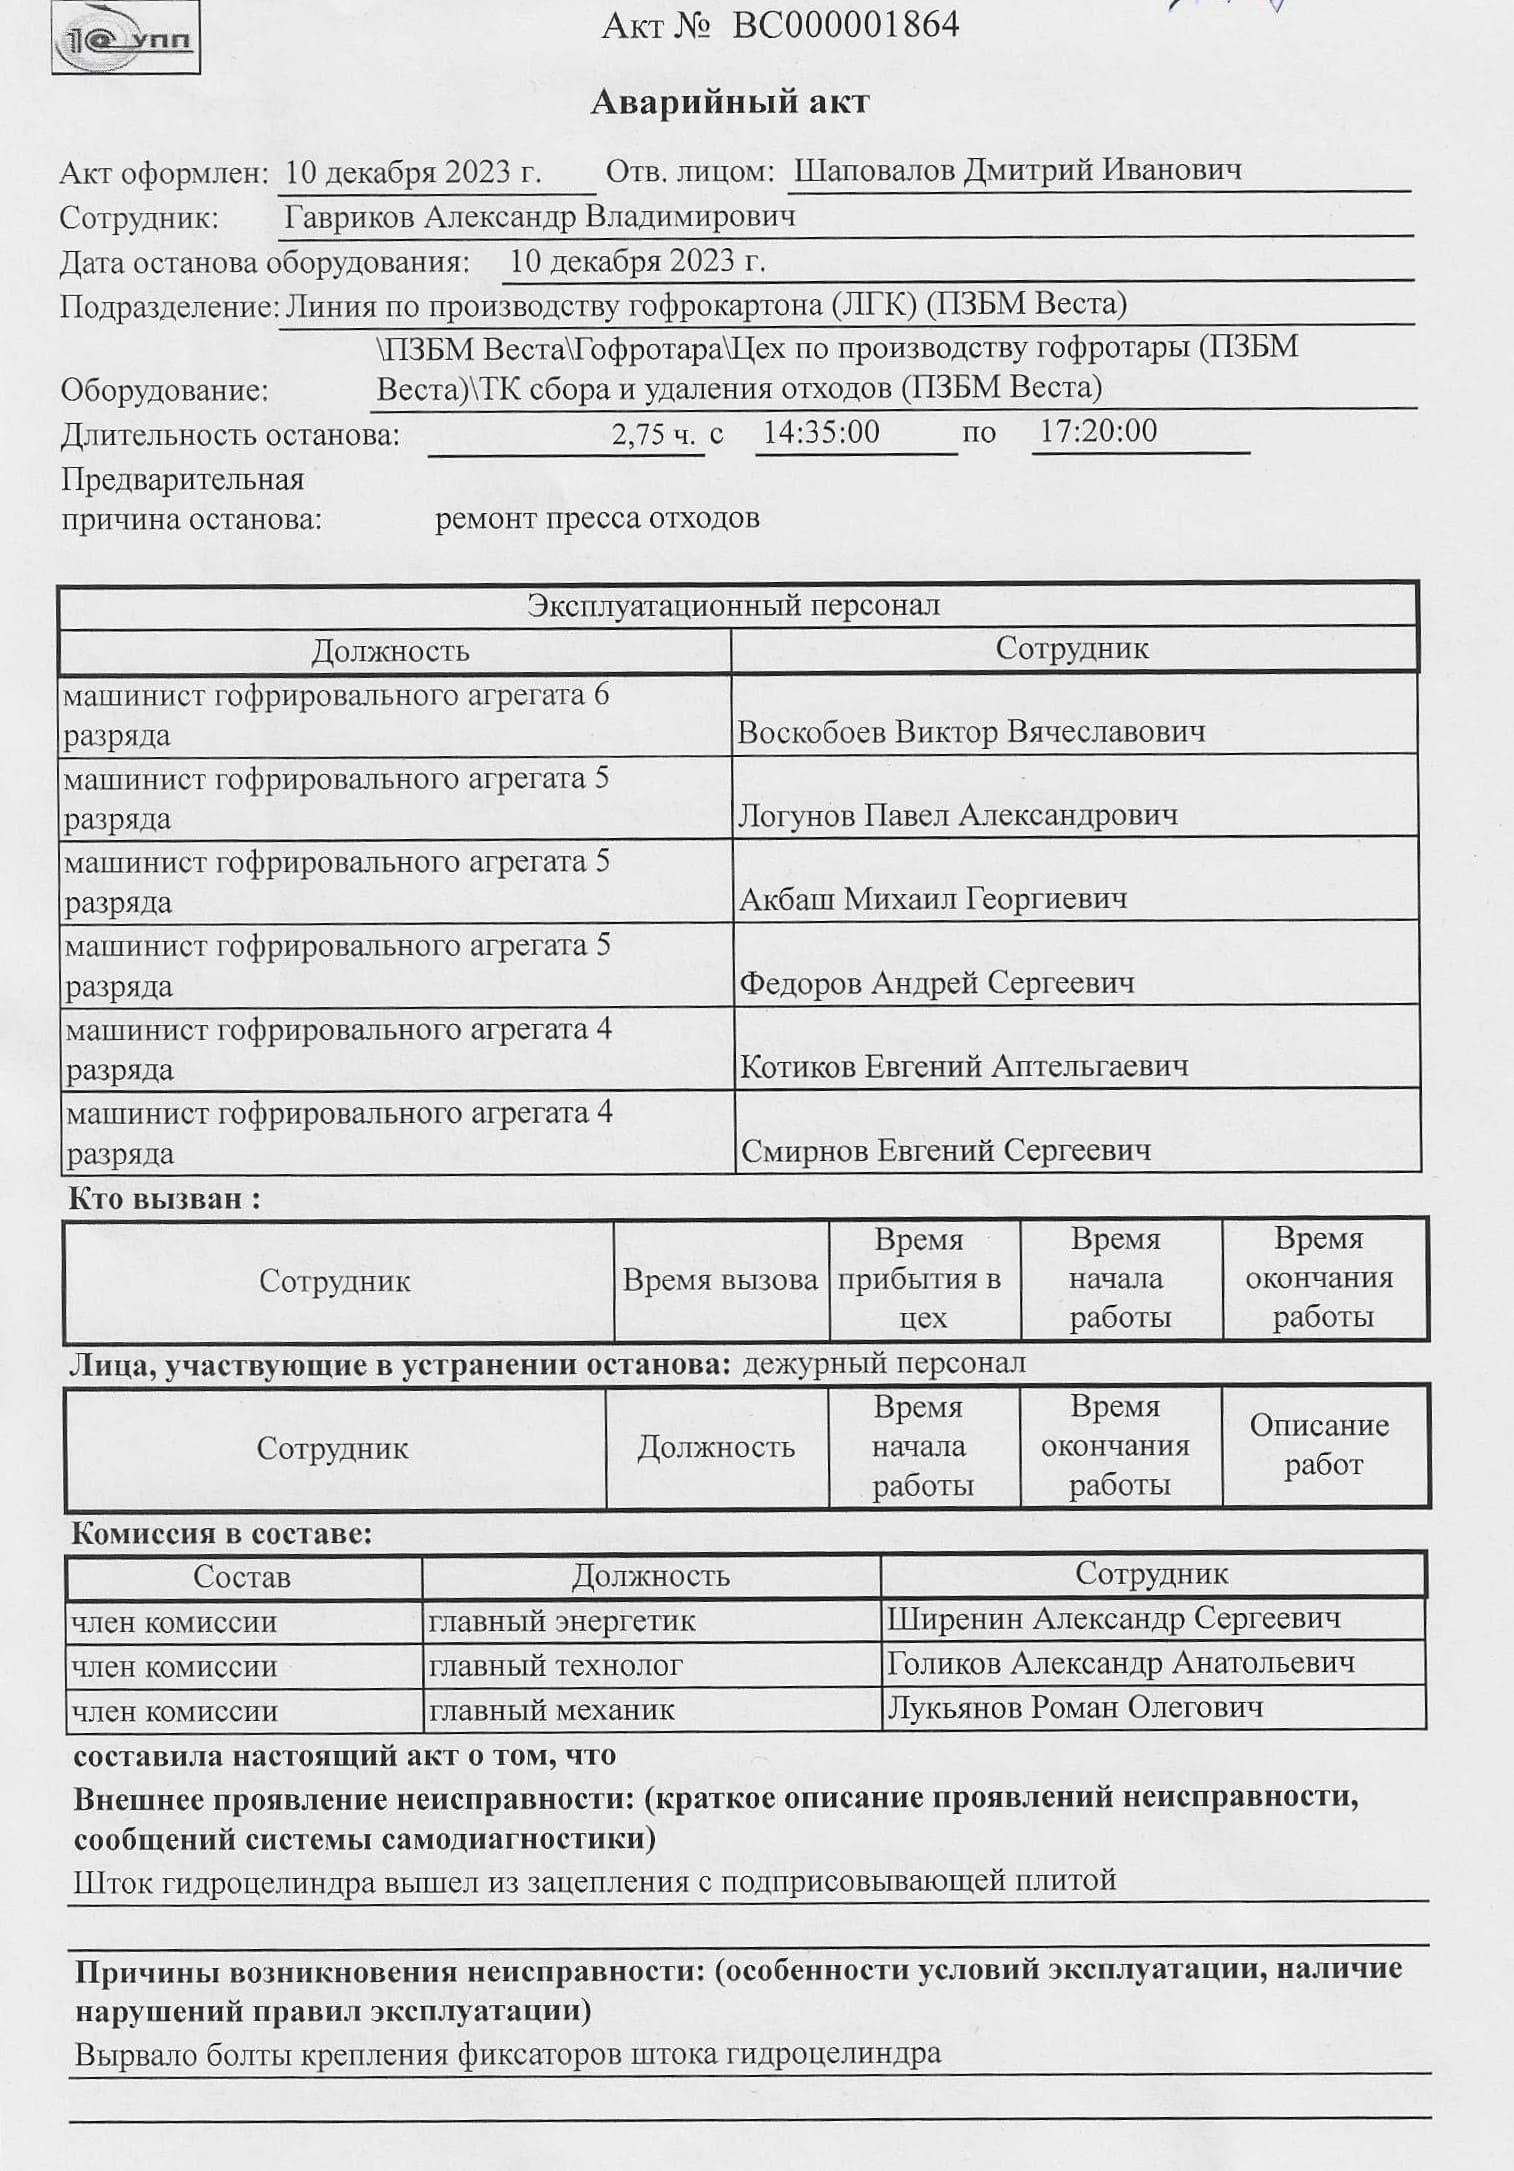
\includegraphics[height=0.9\textheight, keepaspectratio]{Pics/XII.7.jpg}
\end{center}
 \caption{Аварийный акт}
 \label{pic:XII.7.jpg}
\end{figure}

\begin{figure}
\begin{center}
 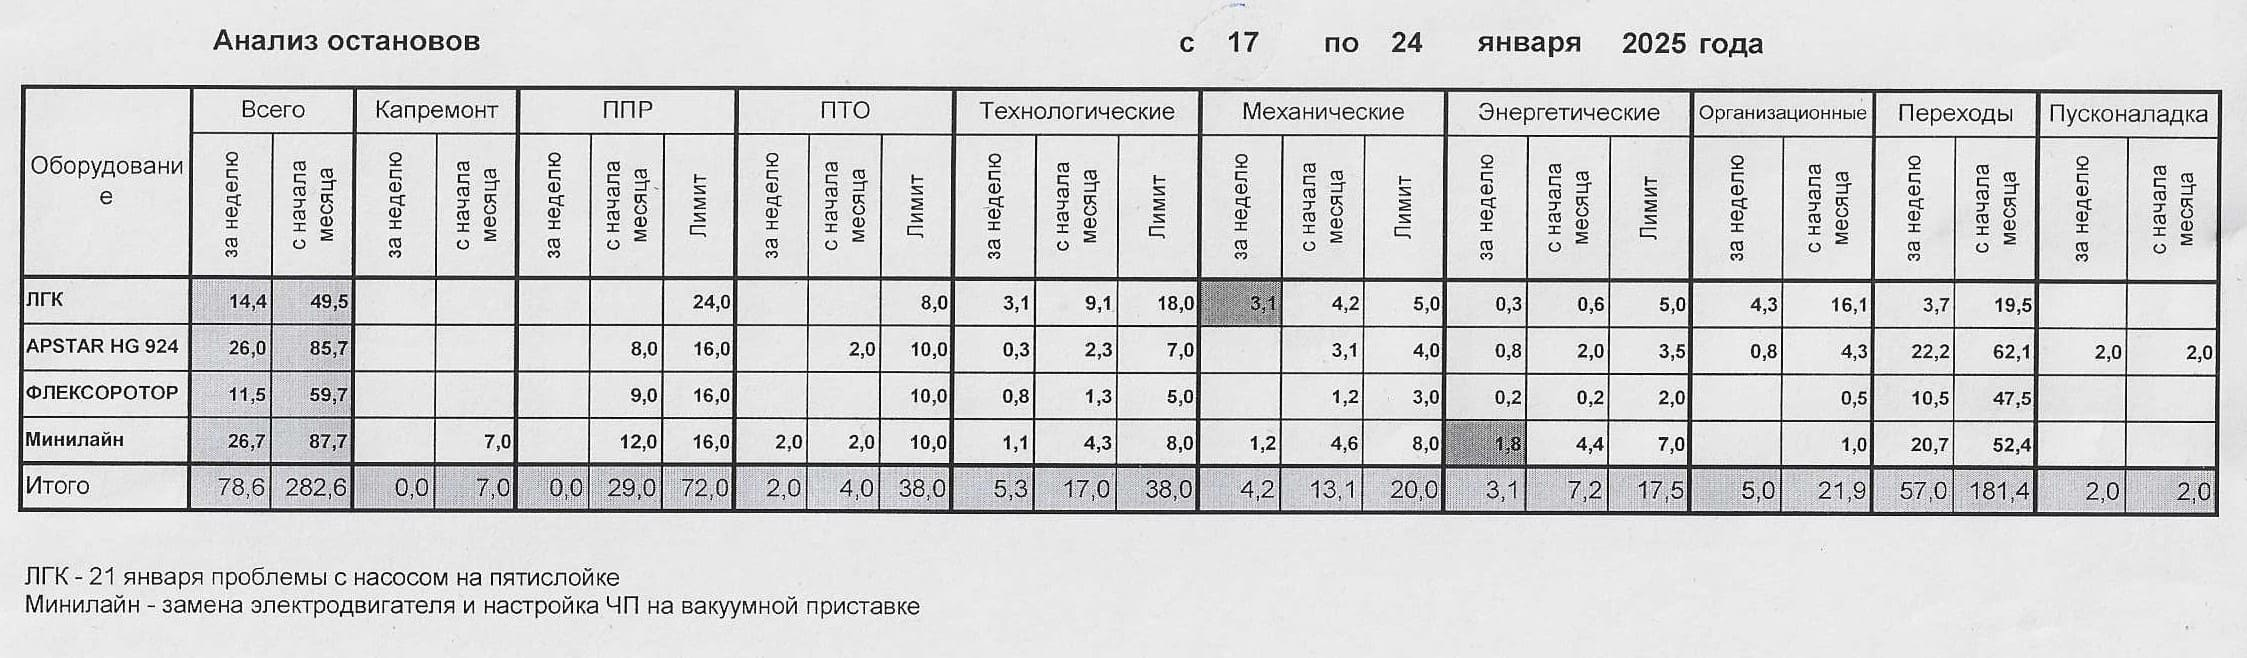
\includegraphics[height=0.2\textheight, keepaspectratio]{Pics/XII.8.jpg}
\end{center}
 \caption{Анализ остановов}
 \label{pic:XII.8.jpg}
\end{figure}
% \begin{figure}
% \begin{center}
%  \includegraphics[height=0.4\textheight, keepaspectratio]{Pics/f47.jpg}
% \end{center}
%  \caption{Замечания по работе оборудования}
%  \label{pic:f47}
% \end{figure}
\clearpage
\ifx \notincludehead\undefined
\normalsize
\end{document}
\fi